\documentclass[11pt]{article}

\usepackage[a5paper,left=2cm,right=1cm,top=1cm, bottom=1.5cm]{geometry}
\usepackage{array}
\usepackage{makecell}
\usepackage[all]{nowidow}
\usepackage{wrapfig}
\usepackage{enumitem}
\usepackage{multicol}

\usepackage{hyperref}
\hypersetup{
    colorlinks=true,
    urlcolor=sokolblue,
    }

\usepackage[czech]{babel}
\usepackage[utf8]{inputenc} 
\usepackage{ellipsis}

\usepackage{fontspec}
\newfontfamily{\tyrs}{Sokol Tyrs}
\newfontfamily{\fugner}{Sokol Fugner}

% \usepackage{lmodern}
% \usepackage[T1]{fontenc} 
\usepackage{anyfontsize}
\newcommand{\titlesize}{\fontsize{56pt}{67pt}}


\usepackage[dvipsnames]{xcolor}
\definecolor{sokolred}{RGB}{228, 5, 33}
\definecolor{sokoldarkred}{RGB}{200, 0, 30}
\definecolor{sokolblue}{RGB}{45, 46, 135}

\usepackage{tikz}
\usetikzlibrary{calc}

\usepackage{fancyhdr}

\fancypagestyle{standard}{%
    \fancyhf{}
    \fancyhead[LO]{%
        \begin{tikzpicture}[overlay,remember picture]
            \fill [color=sokolred] (current page.north west) rectangle ($ (current page.south west) + (1cm,0cm) $);
            \fill [color=sokolred] ($ (current page.north west) + (1.1cm,0cm) $) rectangle ($ (current page.south west) + (1.2cm,0cm) $);
        \end{tikzpicture}
        }
    % \fancyhead[RE]{%
    %     \begin{tikzpicture}[overlay,remember picture]
    %         \fill [color=orange](current page.north east) rectangle
    %             ($ (current page.south east) + (-1cm,0cm) $);
    %     \end{tikzpicture}
    %     }
    \fancyfoot[C]{%
      \begin{tikzpicture}[overlay,remember picture]
        \fill [color=sokolred] ($ (current page.south east) + (-1.5cm,1.3cm) $) rectangle ($ (current page.south east) + (0cm,0.5cm) $)
         node [pos=0.5,color=white] {\large\tyrs{\thepage}\hspace*{0.5cm}};
      \end{tikzpicture}
    }

    \renewcommand{\headrulewidth}{0pt}
    \renewcommand{\footrulewidth}{0pt}
}



\fancypagestyle{uvodnik}{%
    \fancyhf{}
    \fancyfoot[C]{%
      \begin{tikzpicture}[overlay,remember picture]
        \fill [color=sokolred] ($ (current page.south east) + (-1.5cm,1.3cm) $) rectangle ($ (current page.south east) + (0cm,0.5cm) $)
         node [pos=0.5,color=white] {\large\tyrs{\thepage}\hspace*{0.5cm}};
      \end{tikzpicture}
    }

    \renewcommand{\headrulewidth}{0pt}
    \renewcommand{\footrulewidth}{0pt}
}

\fancypagestyle{blank}{%
    \fancyhf{}
    \fancyfoot[C]{}

    \renewcommand{\headrulewidth}{0pt}
    \renewcommand{\footrulewidth}{0pt}
}


\newcommand{\post}[1]{%
\begin{center}
{\huge \tyrs #1}
\end{center}
}

\newcommand{\subpost}[1]{%
\vspace*{12pt}
\begin{center}
{\Large \tyrs #1}
\end{center}}

\newcommand{\signature}[2]{%
  \begin{flushright}
    \textbf{#1}\\#2
  \end{flushright}
}

\newcommand{\luv}{\clqq\kern-0.07em}
\newcommand{\ruv}{\kern0.07em\crqq\kern0.1em}

\usepackage{csquotes}
\DeclareQuoteAlias{german}{czech}
\MakeOuterQuote{"}

\usepackage[normalem]{ulem}


\begin{document}

%% title
\newgeometry{margin=1cm}
\pagecolor{sokolred}
\color{white}
\pagenumbering{gobble}
\begin{center}

\vspace*{\fill}

\includegraphics*[width=0.75\textwidth]{logo-140-vert-white.pdf}

{\titlesize \fugner ZPRÁVY}

{\titlesize \tyrs SOKOLA LIBEŇ}

\vspace*{1cm}

{\large ročník L · číslo 3 · září 2024}

\vspace*{\fill}
\end{center}

\clearpage
\normalcolor
\nopagecolor
\pagenumbering{arabic}

%% úvodník
\pagestyle{uvodnik}
\newgeometry{margin=1.5cm}


{\fontsize{48pt}{57pt} \fugner \color{sokolred} \noindent Úvodník}
\hfill
{\textbf{Zdeněk Lauschmann}} %\raisebox{24pt}{...}


\vspace*{12pt}
\begin{center}
  \textbf{Krátké vzpomínání bývalého náčelníka}
\end{center}

Zakrátko to bude půlstoletí od mého prvního vstupu do libeňské sokolovny. Bylo mi 16 let a brzy jsem začal pomáhat cvičitelům žáků. Tehdejší náčelník a náčelnice odboru ZRTV\footnote{Základní a Rekreaní Tělesná Výchova} František a Marie Kodlovi vedli cvičení žactva tak, jak to znali z~bývalého Sokola, včetně výletů do přírody. Při TJ Meteor dobře fungovala i aktivní seniorská skupina – Věrná garda. Ti všichni také Sokol pamatovali a měli ho hluboko v~sobě. Byla na nich znát jakási zvláštní radost ze společných aktivit, vytrvalá chuť do života. Takto nepřímo jsem ještě před rokem 1989 postupně poznával to, co bychom dnes nazvali sokolský duch. A~toto upřímné, poctivé zaujetí pro dobrou věc se pak dále svobodně rozvíjelo ve všech činnostech obnovené tělocvičné jednoty.

Po prvním novodobém všesokolském sletu v~r. 1994 jsem se po 18 letech v~Libni rozloučil. Celý sletový rok 1993–1994 už jsem totiž dojížděl z~nového bydliště na Barrandově a dále to nebylo únosné. To loučení však pro mě obsahovalo velikou zpětnou radost a také naději do budoucna. Slet vyzněl celkově výborně a naše Libeň vyslala mnoho cvičenců, žáků měla dokonce nejvíc v~celé republice. A~hlavně jsem měl komu předat jak turistický oddíl Jilm, založený 1982, tak i náčelnictví svěřené mi v~r. 1990 Františkem Kodlem: obojí tenkrát převzal nynější starosta Jiří Novák a obojí dovedl výš, přesně v~sokolském duchu.

Závěr mého vzpomínání je také plný radosti, ale i hrdosti. Z~nového sokolského domova v~malé jednotě na Zlíchově, kde se práce rovněž dařila, jsem totiž Libeň stále sledoval. A~viděl jsem, jak vytrvale a nápaditě jde kupředu v~počtech i úrovni, jak také skvostná libeňská sokolovna znovu získává zasloužený secesní lesk. Na každé Vánoční nadílce Jilmu, na každé akademii, při každé akci, kde Libeň figuruje i v~rámci Prahy či ČOS – vždycky se potěším a jsem hrdý na tuto skvělou jednotu. A~ještě něco – na všech 6 sletech od r. 1994 jsem cvičil mužskou skladbu s~Libní – poprvé jako cvičitel a pak vždy jako cvičenec, protože Zlíchov oddíl mužů neměl. Naposled letos, s~mladým, příkladným náčelníkem Josefem Kubištou na sousední značce – bylo mi ctí!

\vspace*{\baselineskip}
\noindent
Hoj vzhůru, pestrý sokole libeňský a – se 140 dobrými roky za sebou – LEŤ DÁL! 


\clearpage

%% termínka

\pagecolor{sokolred}
\color{white}
\renewcommand{\arraystretch}{1.2}

\newcommand{\boxheight}{12.8cm}

\vspace*{\fill}
\post{TERMÍNOVÁ LISTINA AKCÍ JEDNOTY}
\vspace*{0pt}

\begin{center}
\begin{tikzpicture}
  \draw [ultra thick,color=white](0.3cm,0cm) rectangle (12.3cm,\boxheight);
  \fill [color=white] (0cm,0.3cm) rectangle (12cm,\boxheight + 0.3cm)
  node [pos=.5, color=black] {
    \begin{tabular}{l  p{6.5cm}}
      26. 9. 2024 (čt) & 24. ročník Běhu strmého do zámeckého vrchu \\
      27. 9. 2024 (pá) & Noc sokoloven \\
      8. 10. 2024 (út) & plavba kánoí na Pietní akt k~Památnému dni sokolstva do Tyršova domu – pro zájemce z~řad žactva \\
      10. 10. 2024 (čt) & Pietní akt k~Památnému dni sokolstva \\
      12. 10. 2024 (so) & 67. Podzimní Výlet Libeňského Sokola \\
      8. 11. 2024 (pá) & Župní plavecké závody (děti i dospělí) \\
      9. 11. 2024 (so) & Podzimní brigáda v~sokolovně 9–15 h \\
      10. 11. 2024 (ne) & župní sraz cvičitelů \\
      23. 11. 2024 (so) &Tělocvičná akademie Sokola Libeň – 140 let \\
      24. 11. 2024 (ne) & Divadelní představení České nebe  \\
      5. 12. 2024 (čt) & Mikuláš \\
      19. 12. 2024 (čt) & Loutkáři \\
      19. 12. 2024 ( čt) & poslední cvičení v~roce 2024 \\
      2. 1. 2025 ( čt) & zahájení cvičení v~roce 2025 (ještě jsou prázdniny) \\
      3. 1. 2025 (pá) & Silvestr cvičitelů \\
    \end{tabular}
  };
  %  node [color=black] {FOOBAR};
\end{tikzpicture}

\renewcommand{\arraystretch}{1}

\vspace*{12pt}
Podrobné informace k~akcím budou zveřejňovány na našich internetových stránkách a distribuovány dalšími obvyklými kanály (cvičitelé, vývěsky, e-mail)

\end{center}
\vspace*{\fill}

\clearpage
\nopagecolor
\normalcolor

%% normální obsah
\restoregeometry
\pagestyle{standard}


\post{Zpráva místonáčelníka}

\subpost{Jaro a léto v~oddíle žáků a dorostenců}
Od 30. dubna až do prázdnin jsme cvičili venku a věnovali jsme se zejména atletickým disciplínám. Sletoví cvičenci vždy část hodiny věnovali v~sokolovně nácviku a teprve pak se připojili k~ostatním. 1.–2. června se konalo celostátní finále závodů ve všestrannosti mladšího žactva. Z~Libně postoupilo 5 závodníků, dorazit mohli čtyři. V~žactvu obsadil Vojtěch Bőhm 8. místo z~12 závodníků (2. v~plavání, 3. v~atletice, 4. ve šplhu a 11. v~gymnastice). V~mužích obsadil Josef Kubišta 6., Jakub Kudroň 8. a Lukáš Šimek 9. místo mezi 9 soupeři. Jediné medailové umístění získal J. Kubišta ve šplhu, kde byl druhý. 

27. června proběhlo vyhlášení celoročních soutěží žáků. V~zimní soutěži 2024 – shyby mezi 44 mladšími žáky ve svých ročnících vyhráli: J. Nepomucký (4), J. Vandas (5), M. Cakl (10) a L. Bednář (10) a v~celkovém pořadí se ještě dobře umístili:  A. Musil (9), O. Boušek (8), J. Černý (8), F. Gaberle (7), V. Zelený (7), R. Marin (6), F. Vinkler (5), M. Duda (5) a T. Voráč (5). Mezi 35 staršími žáky zvítězili ve svém ročníku: M. Trnka (8), J. Smutný (15), V. Bőhm (16), H. Hőschl (12) a  jmenování si dále zaslouží J. Šefrna (13), F. Novák (11), Š. Novák (10), T. Novotný (10) a S. Budai (9). Mezi 20 dorostenci a cvičiteli byli nejlepší:  J. Kubišta (26), V. Blahunek (15), J. Pikálek (15), T. Kléger (15), P. Boháč (14), D. Vršecký (12), J. Kerhart (12) a A. Basseville (11). Celkem bylo hodnoceno 99 cvičenců. 

V~celoroční soutěži O~nejvěrnější docházku byli nejpilnější tito cvičenci (přijít se mohlo $77\times$): $77\times$ J. Novák, $76\times$ T. Novák, $75\times$ T. Kléger, $73\times$ L. Bednář, M. Sokol, J. Kubišta, $71\times$ A. Musil, $70\times$ K. Jordán, P. Ettel, $69\times$ J. Kerhart, $67\times$ D. Hájek, J. Pikálek, $65\times$ J. Černý, C. Hradečný, J. Doupal, $63\times$ M. Trnka, A. Basseville, $62\times$ A. Příhoda, F. Šefrna, P. Šimčík, Š. Novák, $61\times$ R. Hroz, O. Doupal, $59\times$ J. Vandas, O. Ševčenko, $57\times$ F. Šefrna, $56\times$ R. Marin, J. Novák. Dalších 31 kluků mělo docházku nad 50\,\%. Celkem bylo zapsáno 136 cvičenců (67 mladších žáků, 39 starších žáků, 13 dorostenců a 17 cvičitelů). Celoroční průměr docházky byl 59,84 (minulý rok 52,53) při průměrně měsíčně zapsaných 106,9 (loni 100,7) cvičenců. 

O~víkendu 21.–23. 6. 2024 vyrazily turistické oddíly připravit tábor. Jelo 21 vedoucích a členů Jilmu a Veverek a dále dalších 7 pomocníků převážně z~řad cvičitelů. Vzhledem k~tomu, že na tábor se jelo až za 3 týdny, dělaly se pouze práce a stavby, které tento čas bez problémů přečkají. Posekala se, pohrabala a odvozila tráva z~malé louky kolem kuchyně, vykopaly se jámy na latrínu a odpadovku (u~té se udělalo i víko), postavila se nová lávka u~dřevníku, udělalo se několik nových tyčí na týpka (tj. pokácet soušku a čistě ji osekat od větví), opravilo se slavnostní ohniště, na konstrukce dřevníku a seníku se natáhly a připevnily plachty, opravilo se korýtko včetně schůdků, vyčistil se sklípek a hlavně se postavila střecha kuchyně.

\subpost{Slet}
\textbf{Sletový průvod} zahájil sletový týden v~neděli 30. června za slunečného a parného dne. Okolo desáté jsme se seřadili v~dolní části Václavského náměstí. Následně se jako první dala do pohybu Sokolská stráž s~prapory, dále sokolové ze zahraničí, pak všechny mimopražské župy a nakonec župy pražské jako hostitelé sletu. My jsme tedy do trasy průvodu vyráželi až kolem jedenácté. Na trase, která vedla po Národní třídě, kolem Národního divadla, po nábřeží okolo Rudolfina a pak Pařížskou ulicí na Staroměstské náměstí, nás zdravily zástupy diváků a hrály sokolské hudby. Z~Libně šlo celkem 172 cvičenců, z~toho přes 40 bylo zásluhou vzdělavatelky Anky Holanové v~historických krojích či historických cvičebních úborech. Krátce po poledni průvod skončil a my se rozešli domů a čekali na pondělí, kdy začnou secvičné zkoušky v~Edenu.

\textbf{Zkoušky skladeb} probíhaly v~areálu Slavie v~Edenu od pondělí do čtvrtka jednak na fotbalovém sletovém stadionu, ale i na menší ploše stadionu atletického. Každá skladba měla nejprve dvě zkoušky samostatně, pak následovala takzvaná projížděčka každého z~obou programů a nakonec byly i generálky obou programů. Takže ve středu a ve čtvrtek se tam muselo dojet třikrát. A~pak už nás čekala jen vlastní vystoupení.

Během sletového týdne jsme si užili také \textbf{Sokol gala} – komponovaný program odboru sportu, který se konal v~O2 aréně v~úterý 2. července. V~moc hezkém skoro dvouhodinovém programu nebyly k~vidění jen ukázky sportů (trampolína, různé tance, šplh, šachy, krasojízda, volejbal, košíková, gymnastika, závěsná akrobacie, teamgym, zápas, box, judo, capoeira), ale došlo i na vystoupení Hradní stráže, sletové skladby mužů Před kamerou, akrobatické vystoupení Sokolské stráže a cvičení hostů z~Amerického Sokola. To vše doprovázeno živou kapelou a zpěváky a zasazené do historického rámce a vývoje Sokola. Spousta věcí byla promítána na kostce nad plochou. Moc hezké představení to bylo. Škoda jen, že ho řada z~našich členů nemohla navštívit, neboť jsme dostali většinu lístků na odpolední generálku, kdy probíhaly v~Edenu zkoušky skladeb (např.  mužů). 

\textbf{Sletová vystoupení} byla dvě. Jedno večerní od 21 hodin skoro do půlnoci ve čtvrtek 4. 7. a druhé odpolední v~pátek 5. 7. od 14 do 17 hodin. Večerní vystoupení bylo bohužel stejně jako před šesti lety poznamenáno deštěm. Cvičenci zmokli již při příjezdu do Edenu, pak na seřadišti a první skladby včetně zahájení s~prapory i na ploše. Navíc místa pro cvičence na stadionu byla v~prvních řadách, kam i přes zastřešení tribun pršelo. Mokří jsme tak byli všichni. A~kdo z~cvičenců chtěl vidět vystoupení jiných skladeb naživo jako divák na stadionu, tak si pěkně zaběhal. Ze šaten 500 m po ulici na stadion. Pak stejnou trasou zpět do šaten a na seřadiště. Přesun na stadion, odcvičení vlastní skladby, 500 m běhu k~šatnám a východu z~areálu, dalších 500 metrů po ulici na tribunu. A~kdo měl na starosti dětskou skladbu a zároveň cvičil i skladbu pro dospělé, naběhal se dvakrát tolik. Ale stálo to za to. Všechny skladby byly moc pěkné, a to i ty, které se nám po prvním zhlédnutí instruktážních videí na podzim 2022 moc nepozdávaly. Stadion na pátečním programu byl vyprodaný a diváci neuvěřitelně přející. Hodili jsme za hlavu všechny nedostatky, kterých se organizátoři vůči cvičencům dopustili (a nebylo jich letos málo – pozdní informace, vstupenky sokol gala většinou na odpolední generálku, příšerné ozvučení na seřadišti a během zkoušek, vyřazení skladby Fitness z~programu Sokol gala 12 dní před vystoupením, tragická doprava po večerní generálce a vystoupení z~Edenu na Palmovku atd.) a užívali si společný úspěch a radost z~toho, že to, čemu jsme věnovali posledních pár měsíců, stálo za ta příkoří.

Náš \textbf{posletový táborák} se konal hned po skončení odpoledního vystoupení, kdy jsme se přesunuli z~Edenu k~sokolovně, zapálili oheň, posedali si na připravené lavičky, zazpívali pár písniček, poslechli si hodnocení sletu z~úst starosty, náčelníka a některých dalších cvičitelů. Byla spousta děkování. Rodičům za trpělivost během celého nácviku i sletového týdne, cvičencům za hezké zacvičení, cvičitelům, kteří je to naučili atd. Během táboráku došlo i na rozdání pamětních medailí, které naše jednota nechává vyrobit po každém sletu pro své cvičence. Také došlo na symbolickou odměnu šestnácti hlavním cvičitelům a vzdělavatelce za starost o~nácviky sletových skladeb a sletový průvod (ručník, pantofle do sprch, poukázka do sportovního obchodu). Následně jsme si opekli buřty, zjistili skutečný počet libeňských cvičenců na sletu – \textbf{240 jmen, 274 značek!} Zdaleka nejvyšší čísla od obnovení Sokola v~roce 1990. Vždy jsme byli nad 100 účastníky, v~roce 2018 byl prozatímní vrchol (146 cvičenců, 166 značek), ale tentokrát takový obří skok, za který jsme ale moc rádi. Ale kam se hrabeme třeba na rok 1920, kdy z~Libně vystupovalo mimo jiné třeba 320 vybraných mladších žáků. 

Sešlo se nás u~ohně okolo 170 vesměs spokojených cvičenců a rodičů. Řada z~nás už viděla večerní vystoupení v~televizi a doporučovali jsme zhlédnutí sletu v~televizi i těm, kteří tak zatím neučinili. Aspoň budeme vědět, jak ta naše skladba vypadala z~pohledu diváka. A~když odhlédneme od chabého výkonu moderátorů, byla to hezká podívaná. Tak zase za šest let. A~třeba nás už bude přes 300. A~pro malé připomenutí je možné si v~přízemí sokolovny prohlédnout hromadná fota jednotlivých skladeb i pár fotografií z~vystoupení, průvodu, táboráku a programu Sokol gala.

\subpost{Letní tábory}
V~létě se naše turistické oddíly vydaly na své tábory do Tajanova u~Velhartic. 

Nejprve se o~víkendu 19.–21. 7. za účasti 23 pracantů z~řad Jilmáků, bývalých Jilmáků a jejich rodinných příslušníků, Veverek a dalších ochotných pomocníků tábor po červnové pracovce kompletně dostavěl – dokončila se latrína, kompletně se vybavila kuchyně, dokončil dřevník, opravil seník, postavil se zásobák, stany a týpka, vztyčil se stožár, postavila brána a zábradlí, umylo nádobí, drobné vybavení se roznosilo do příslušných stanů (léky, kancelářské potřeby, knihy, hudební nástroje, nářadí, celty, hry, sportovní potřeby atd.).

Pomocníci v~neděli večer odjeli a začal \textbf{Tábor bývalých členů} – 22.–27. 7. Celkem bylo 19 osob, z~toho 7 bylo Jilmáky. Užili jsme si pohodový týden za velmi příjemného počasí i s~výletem na Kleť, Dívčí kámen, do Českých Budějovic a na nové tábořiště nedaleko Trhových Svin. Další na řadu přišla \textbf{Káňata} v~termínu 27. 7. – 10. 8. Během 14 dní pobytu se vystřídalo 5 vedoucích, dále byla tři děvčata z~Veverek jako pomocníci vedoucích a 12 dětí. Nakonec přijeli na poslední 3 týdny prázdnin \textbf{Jilmáci a Veverky} na společný tábor. Prostřídalo se 9 vedoucích a bylo 19 dětí (15 kluků a 4 holky).

O~posledním víkendu 30. 8. – 1. 9. přijelo pomoct 18 pomocníků z~řad cvičitelů, bývalých členů, rodičů apod. s~bouráním tábora. Vše proběhlo nečekaně rychle, takže již v~sobotu večer bylo vše vzorně rozebráno, uskladněno ve stodole nebo naloženo v~autech a vozících. Nedělní návrat se tak posunul z~nedělního pozdního odpoledne již na poledne. Všechny tábory se líbily, počasí bylo spíše parné, občas bouřka, všichni se vrátili zdrávi a s~hezkými zážitky. 

Celkem tedy 6 týdnů táborů s~68 táborníky (27 dospělých a 41 dětí).

\subpost{Podzim v~oddíle žáků a dorostenců}

\begin{center}
  \noindent\textbf{Organizační informace}
\end{center}
\vspace*{6pt}
Mladší žáci (2015–2018) cvičí v~út a čt v~17–18 h, st. žáci a dorostenci (2007–2014) v~út a čt v~18–19 h. Pro cvičitele a dorostence je možnost úterního cvičení mužů a čtvrteční košíkové (vždy 19–20).

Pevně věříme, že kluci i díky Vám přivedou další nové kamarády – i když docházka zatím vypadá slibně. Na první úterní hodině 67 kluků, ve čtvrtek 69 a již 15 nových tváří, ale rádi uvítáme další zájemce o~cvičení (bereme mladší i starší žáky). Děkujeme a těšíme se. Doufáme, že v~nadcházejícím cvičebním roce se s~průměrem dostaneme už nad 60.

V~září a začátkem října budeme cvičit opět venku (v~parku u~Rokytky a na zahradě sokolovny). I~ven se nosí stejný cvičební úbor jako do tělocvičny – modré trenky a bílé tričko se sokolským znakem. Na nohy je nutná vhodná zavazovací obuv (sandály opravdu nejsou atletické či fotbalové obutí). Jen v~případě deště a velmi chladného počasí se bude cvičení konat v~sokolovně. Nenavlékejte na kluky zbytečně tepláky a mikiny – pohybem se dostatečně zahřejí a drobné otužování upevní jejich zdraví. 

Zdůrazňujeme, že začátek i konec cvičení je v~šatně – děkujeme. Pokračuje jarně-podzimní soutěž Letní disciplíny (atletika) a opět začíná celoroční soutěž O~nejvěrnější docházku s~pravidelným každoměsíčním vyhlašováním a rozdáváním diplomků za 100\% docházku. 

Od 8. října budeme cvičit už jen v~sokolovně – kromě gymnastiky nás tedy čekají i vnitřní hry a též nácvik na Akademii. Připomínáme také, že za pozdní příchod či absenci úboru vybíráme pokutu 1 Kč (do fondu odměn za docházku). 

O~podzimních prázdninách 29. 10. žáci cvičí.

O~kluky se bude starat náš mužský cvičitelský sbor v~tomto složení:

Cvičitelé: J. Novák (54), T. Novák (52), J. Kudroň (36), J. Přibyl (33), J. Kubišta, (32), D. Unzeitig (24), J. Kerhart (22), P. Boháč (21) a naši mladí pomahatelé: J. Skokan, T. Kléger, V. Novák, V. Blahunek, J. Pikálek a A. Basseville. Od října, až se ustálí počty žáků a rozvrhy studujících cvičitelů, dostane každé družstvo žáků (děleno dle ročníků narození) své stálé cvičitele. V~říjnu a listopadu vyšleme na školení cvičitelů další zájemce.

Výsledky závodů, fota, dopisy a další informace najdete na vývěskách v~sokolovně a na ní a také na www.sokol-liben.cz.


\vspace*{12pt}
\begin{center}
  \noindent\textbf{Příspěvky}
\end{center}
\vspace*{6pt}
S~placením příspěvků prosím vyčkejte, dokud vám nepřijdou e-mailem platební instrukce ze systému EOS. Bude to okolo 15. září. Do té doby musíme cvičence přesunout do správného oddílu a zjistit, kolik hodin týdně chodí. Pokud přesto někomu přijde platba za špatný oddíl či za jiný počet hodin, přihlašte se do systému EOS, dejte \luv{}Nový požadavek na management\ruv{} a tam napište aktuální údaje. Původní platba bude stornována a následně vám přijde správná. Prosíme o~zaplacení příspěvků na druhé pololetí roku 2024 nejlépe do konce září a přes účet (žáci cvičící $1\times$ týdně 1 475\,Kč, žáci cvičící $2\times$ týdně 1 850 Kč). Zcela noví kluci se musí přihlásit – na stránkách dáte odkaz na systém EOS, kliknete na nová přihláška, vyplníte základní údaje (jméno, datum narození, oddíl a počet hodin týdně) a odešlete. Systém vám do 24 hodin pošle kompletní přihlášku. Tu vyplníte a odešlete. V~řádu dní vám přijdou instrukce k~platbě příspěvků. Bližší informace k~vyplňování přihlášky naleznete v~návodu na našich internetových stránkách. 

V~matrice – 1. patro sokolovny (čtvrtek 15:45–18:45) lze pak zakoupit bílé tričko se znakem nebo znak na vlastní bílé tričko. Všechny, kteří již v~minulosti přihlášku za sebe či svoje děti vyplnili a odevzdali, prosíme, aby se zamysleli, jestli nedošlo k~nějaké změně (kontakty, zdravotní stav, \ldots), a pokud ano, aby údaje v~systému EOS aktualizovali – děkujeme.

\vspace*{12pt}
\begin{center}
  \noindent\textbf{Nabídka dalších aktivit}
\end{center}
\vspace*{6pt}
Všem žákům nabízíme možnost účasti na výletech, které pořádají naše turistické oddíly. Jilm a Veverky mají společný program a zvou starší žáky a žákyně (kluky a holky 9–14 let). Schůzky jsou ve středu v~klubovně. Výpravy se konají cca $1\times$ měsíčně. Vyvrcholením celoroční činnosti je pak letní tábor. V~roce 2025 to bude na novém místě u~Trhových Svinů. Podařilo se nám udržet také činnost Káňat, kde se potýkáme s~nedostatkem vedoucích.

Líbí se vám cvičení mužů na akademiích? Klidně se můžete stát členem oddílu – berou další zájemce (muže 18–50 let). Cvičí se v~úterý v~19–20. 

Výborně funguje také před několika lety založený oddíl šplhu (osmimetrové lano ze sedu bez přírazu). Řada jeho členů se účastní i mistrovství republiky v~tomto sportu. Též berou další zájemce od staršího žactva až po muže a od loňska šplhají i děvčata a ženy. 

Další větví v~mnohotvárné činnosti mužů je přetah lanem – i v~tomto sportu se závodí a konají se i mezinárodní soutěže. 

\vspace*{12pt}
\begin{center}
  \noindent\textbf{Plánované akce}
\end{center}
\vspace*{6pt}
Čtvrtek a pátek 13.–14. 9. 2024 – pronájem sokolovny na setkání pracovníků firmy Emil Frey k~100. výročí založení jejich firmy. Kromě pronájmu se částečně budeme podílet i na programu pro účastníky (vystoupení akrojógy, Skipping Buddies, sletové skladby Sokolhraní, organizace sportovních zápasů a cvičení na nářadí, loutkové divadlo, dětský koutek atd.). Další finanční přilepšení jednotě mimo jiné i prací našich členů a cvičitelů. Mělo by nám to vynést cca 100 000 Kč.   

Čtvrtek 26. září – \textbf{24. ročník Běhu strmého do zámeckého vrchu} od 16:30 do 18:30. Běží se 199 metrů s~převýšením 29 metrů v~libeňském parku. Přijďte všichni, ať překonáme rekord v~počtu účastníků (204) a trénujte, aby padl i rekord trati 36,25 nebo rekord vaší kategorie. Vyhlášení výsledků v~19:00 v~místě startu. 

Cvičitelé se po Běhu strmém sejdou na pracovní schůzce, kde si rozdělí pořadatelství akcí a další úkoly.

Pátek 27. nebo sobota 28. září – \textbf{Noc sokoloven}. Tentokráte je tématem šplh ve vzpomínce na zlatou medaili Bedřicha Šupčíka na olympiádě v~Paříži v~roce 1924.

V~úterý 8. října je v~kalendáři \textbf{Památný den sokolstva}. Pokud se najde dostatečné množství cvičitelů, budou moci zájemci z~řad Jilmu a sletových žáků vyrazit na kánoích po Rokytce a následně proti proudu Vltavy přes zdymadlo na Štvanici do Čertovky u~Tyršova domu, kde proběhne pietní akt. Pro zájemce s~bicykly nabízíme Spanilou jízdu sokolstva od krematoria Strašnice k~Tyršovu domu, kterou organizuje župní vzdělavatel br. Richter. U~nás v~sokolovně proběhne vzpomínka na umučené sokoly za druhé světové války ve čtvrtek 10. 10. 2024 od 18:00 s~proslovy, písněmi, květinami u~pamětní desky v~sokolovně a vypuštěním lodiček se svíčkami na Rokytce. Zveme veškeré členstvo.

\textbf{Podzimní Výlet Libeňského Sokola} (již 67. v~pořadí) bude v~sobotu 12. října. Opět se připojíme ke Srazu v~přírodě pražských žup. Bude na nás čekat Modrá stuha a různé hříčky, budou i Pamětní lístečky, Písnička a další tradiční součásti setkání. Bližší informace ve zvláštním dopisku koncem září. S~sebou jídlo a pití na celý den, odpovídající oblečení, peníze na jízdné a srazový příspěvek. Těšíme se na hojnou účast v~barevné podzimní přírodě.

Pokračovat budou akce ke 140. výročí založení Sokola Libeň. Sledujte naše stránky a zprávy ze systému EOS, kde budeme postupně uveřejňovat podrobnosti k~jednotlivým akcím. 

Teď se na nové žáky v~Sokole těší a do podzimu pevné zdraví přeje

\signature{Jiří Novák (Jirkan)}{místonáčelník\\tel.: 602 284 198}


\clearpage

\newgeometry{margin=0pt}
\pagestyle{blank}
\begin{center}
  \noindent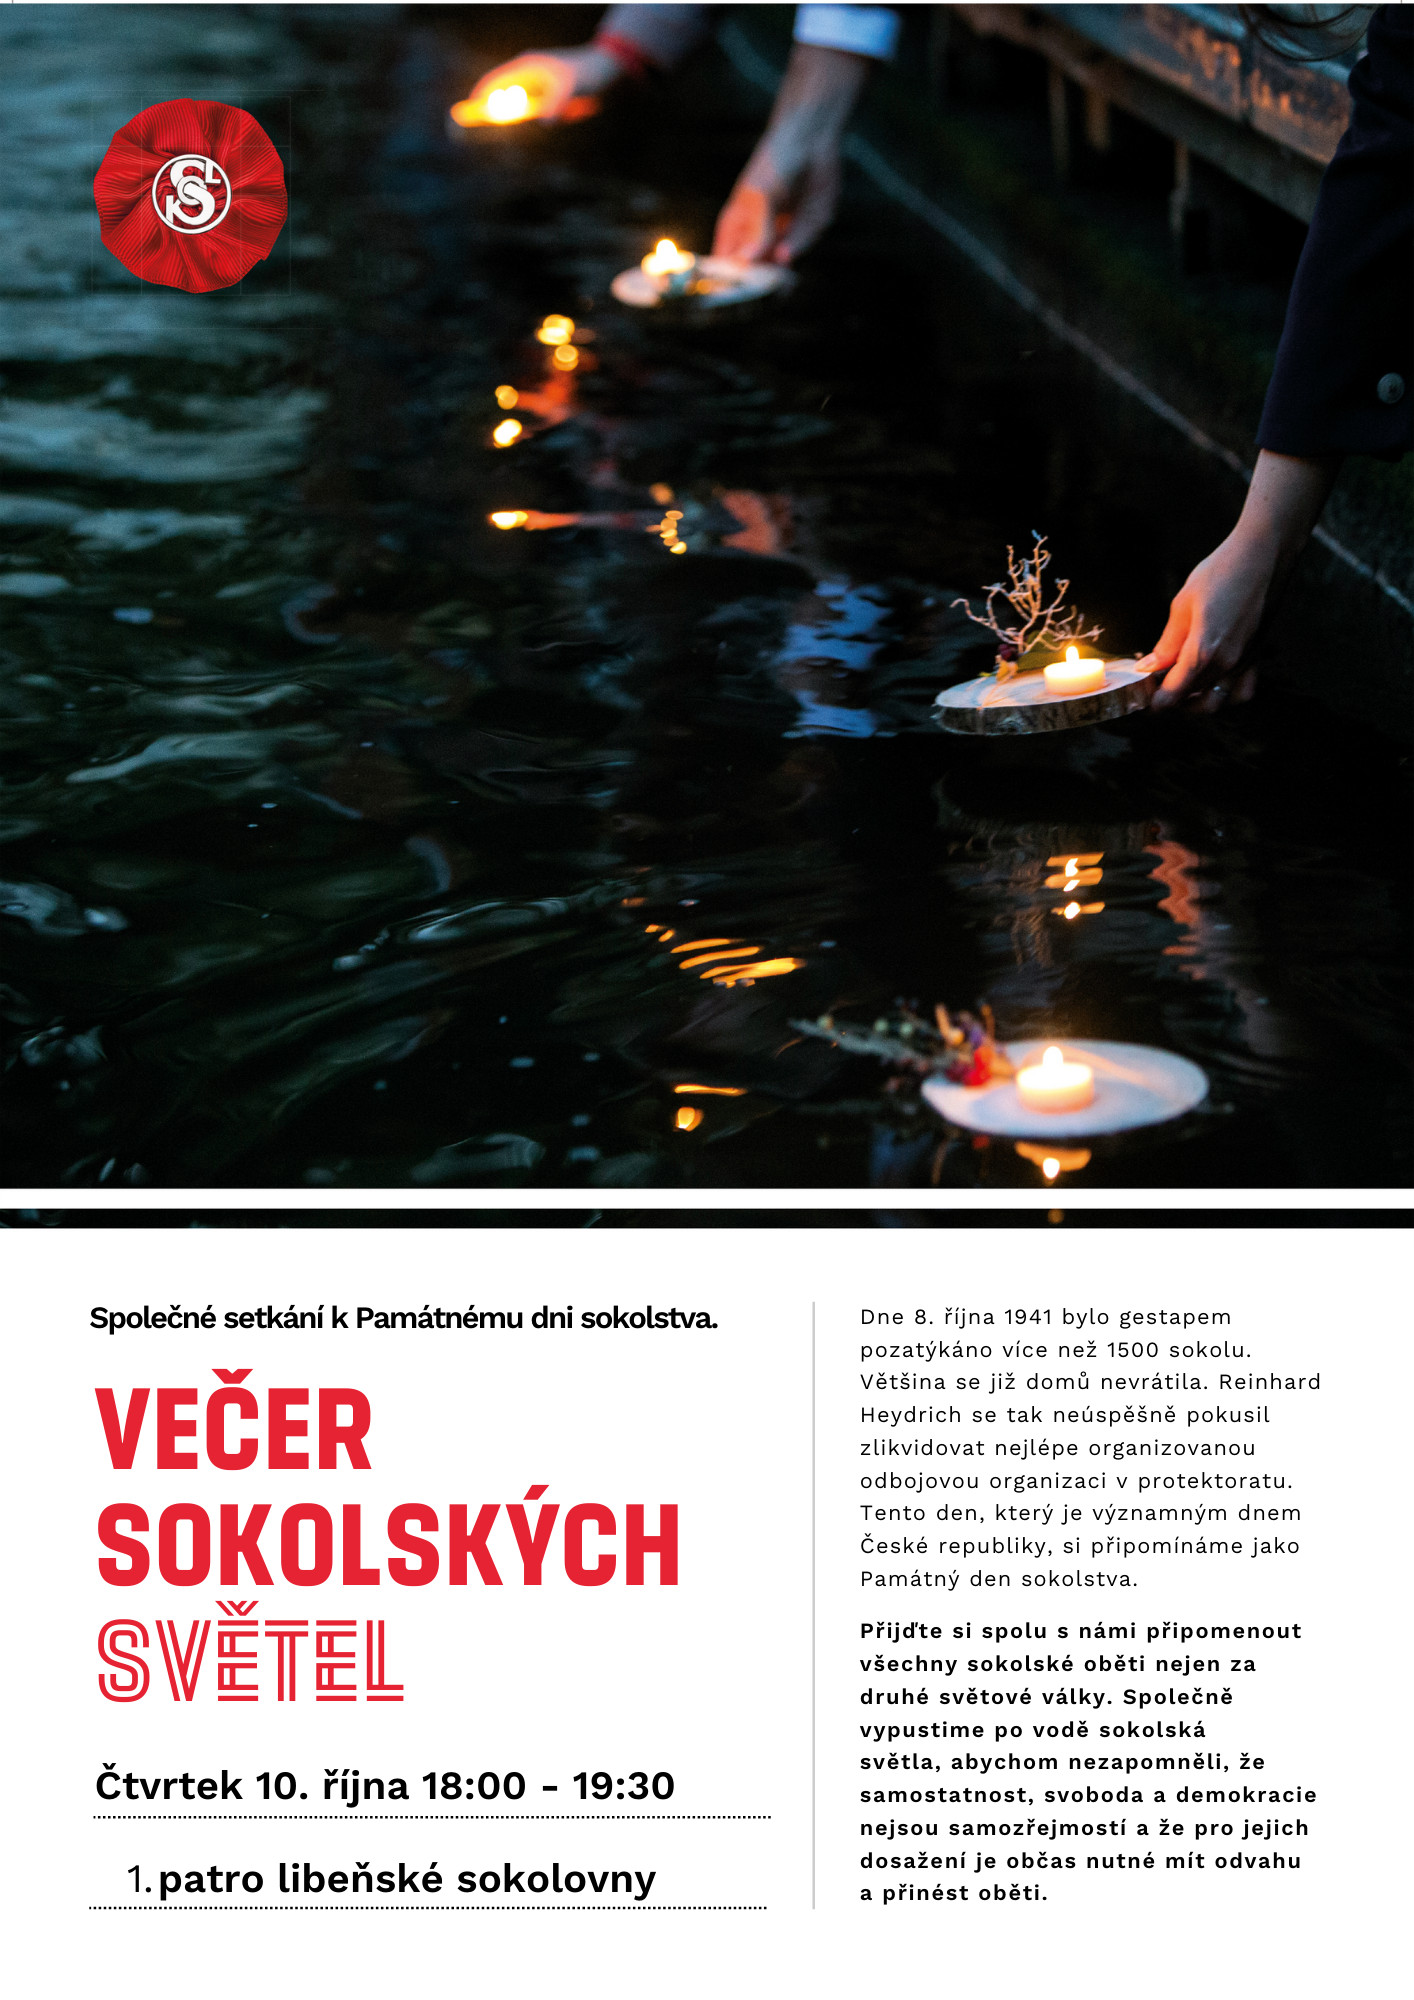
\includegraphics[width=\linewidth]{pamatny-den-sokolstva.jpg}
\end{center}
\restoregeometry

\clearpage
\pagestyle{standard}


\post{Informace od starosty}

Od posledních Zpráv jsme opět kousek pokročili jak v~údržbě sokolovny, tak ve zlepšování naší finanční situace. Co zůstává stabilní, je počet členů, který je stále okolo 800.

Přes léto se podařilo uskutečnit malé vylepšení šatnových skříněk (netýká se těch o~poloviční výšce, které jsou určené pouze pro jednorázové odložení věcí) – byly vyřezány otvory ve spodní a zadní či vrchní části skříněk, které byly osazeny větracími mřížkami. Uložené věci by tak měly lépe vysychat.

Již jsou ve výrobě držáky na lavice do prostoru vedle schůdku do sprch a během podzimu dojde k~jejich namontování a osazení fošnami na sezení v~provedení jako u~šatnových skříněk a s~deskou s~háčky jako v~šatnových klecích.

Finanční situace jednoty se již stabilizovala díky příspěvkům za I. pololetí roku 2024 a také díky financím z~grantů. Již jsme dostali 518\,000\,Kč z~magistrátu na provoz, od Prahy 8 jsme obdrželi 770\,000\,Kč na cvičení dětí, 40\,000\,Kč na tábory a 35\,000\,Kč na loutkové divadlo a oslavy 140 let. Z~národní sportovní agentury pak přišlo 335\,340\,Kč na provoz a odměny cvičitelů. Dále jsme dostali z~ČOS 18\,000\,Kč na prapor mužů a 5\,000\,Kč na loutkáře. Celkem tedy hezkých 1\,721\,340 Kč. Momentálně máme na účtu cca 1 milion Kč (minimální částka, kterou tam chceme mít) a navíc čekáme, že po zaplacení příspěvků na II. pololetí roku 2024 přibyde dalších 850\,000\,Kč, a také nájemci dodají cca 750\,000\,Kč za část 3. a celé 4. čtvrtletí roku 2024.

I~tak ale výbor už v~dubnu rozhodl a navýšení příspěvků od září v~jednotné výši o~200\,Kč na pololetí (s~drobnými výjimkami – turistické oddíly pouze o~50\,Kč, senioři o~100\,Kč a senioři nad 80 let bez zvýšení). V~ruku v~ruce s~tím jde i zvýšení nájmu školám, nesokolským oddílům i zvýšení režijních poplatků menších sokolských oddílů, a to o~cca 10\%. Již v~lednu byly zvýšeny nájmy nebytových prostor taktéž o~10\%. Tím máme pokryty každoměsíční výdaje, které bohužel průběžně rostou: zálohy na plyn, elektřinu a vodu ve výši 125\,000\,Kč a výdaje na platy zaměstnanců ve výši 165\,000\,Kč.

V~červenci jsme podali daňové přiznání. Kvůli štědrým grantům, které sanovaly naše náklady, a poměrně slušným ziskům od nájemců nebytových prostorů byla daň poměrně vysoká – cca 225\,000\,Kč. Díky tomu ovšem můžeme dále pracovat na zvelebování sokolovny a jejího okolí.

Na jaře nám byla nabízena fixace energií na 2 roky za poměrně nevýhodnou cenu, to jsme odmítli a zůstali na měsíční fixaci. Nyní však přišla nabídka na fixaci půlroční (říjen–březen) za cenu, která je nižší než cena na září a říjen, a tu jsme přijali.

Firma Wandel nám již připravila projekt na propojení staré matriky s~nájemcem ABA Strategie a v~půlce června podala žádost o~stavební povolení. Za chvíli bude půlka září a ani za 3 měsíce povolení nemáme. Lhůta je přitom 30 dní. Nesedíme však s~rukama v~kapsách a už jsme si nechali udělat elektřinu (zásuvky, nové osvětlení) a přívod vody a odpady a instalovali umyvadlo. Firma už si objednala dveře a čekáme, až budeme moci kopnout. Škoda je, že jsme to chtěli mít hotové nejpozději na konci srpna a od září pronajmout. Každý měsíc teď budeme přicházet o~necelých 12\,000\,Kč.

Při té příležitosti byla též vyklizena bývalá místnost uklízeček v~chodbičce ke staré matrice a nainstalováno umyvadlo a výlevka a místnost se po letech, kdy sloužila jako sklad firmy Direkta, opět stane zázemím pro uklízečky v~přízemí sokolovny.

Byla dokončena úprava osvětlení na půdě a také byl namontován nový plech na štítovou zeď, který byl stržen při červnové vichřici.

V~brzké době budeme muset opravit nízkou zídku z~kyklopského zdiva pod plotem hřiště gymnázia, kde vypadává spárovací omítka i celé kameny.

Snad posledním problémem je řešení potíží s~kolaudací podzemní místnosti, při které došlo k~nějakému šumu v~dokumentaci a obdržení negativního stanoviska od památkářů ke kolaudaci. V~závazném stanovisku památkářů se píše, že se vydává na základě předložené projektové dokumentace ke stavebnímu řízení, a tak i bylo vydáno stavební povolení, které jsme od architektů měli objednáno na klíč. Na památkářích je však zaevidováno toto povolení na studii, která předcházela projektu, a stavba tam vypadá odlišně. Takže bylo vydáno ono negativní stanovisko. Architekti uznali svoje pochybení, na památkáře bylo zaslána žádost o~stanovisko k~projektu, kde jsou nějaké podmínky – třeba jiný vzhled vnějších stěn místnosti a zídky. Práce byla u~architektů reklamována, škoda činí cca 350 000 Kč a tu po archicraftu požadujeme. Momentálně řeší archicraft se svojí pojišťovnou. V~tuto chvíli zatím nemáme volné finance na předělání a stavebně se to nejspíše bude řešit až v~roce 2025. Pak by snad už mohla být místnost zkolaudována.

Do nové místnosti nám firma Juhász vyrábí držáky na kánoe a kajaky (už je svařeno a čeká se na pozinkování), které v~průběhu podzimu i namontuje. Na podzimní brigádě tak dojde k~přestěhování zbylých věcí ze staré garáže a ta se bude rozebírat (některé části pravděpodobně použijí turistické oddíly pro vybudování úložiště podsad a dalšího vybavení na novém tábořišti).

Na jarní brigádě by pak mohlo dojít k~rozbití a odvezení starého betonu, úpravě povrchu a následnému zatravnění plochy po staré garáži.

Koncem srpna se v~naší sokolovně neformálně sešlo předsednictvo ČOS k~jednání – nový starosta Martin Chlumský – Čedok (náš dlouholetý člen a cvičitel) pozval své kolegy do domovské jednoty.
Jako každý rok se už od jara pilně starám o~nechtěnou (plevel) i žádanou (trávník) zeleň kolem celé sokolovny a snad je to trochu vidět.

\subpost{K~provozu šaten}
Pro začátek prosba k~provozu nových šaten:

Pokud si nechci boty zamykat, použiju poličku, pokud ano, použiju malý zamykací šuplík a zamknu ho.

Větší šuplíky jsou určené pro dětské oddíly, kam se vejde více párů bot. Tak nám je, prosím, neobsazujte vaším jedním párem – děkujeme. Prázdné šuplíky nechávejte odemčené a klíčky vracejte na háček.

Postrádáme klíčky od botníku s~číslem 41 nebo 63. Ty už nám nějaký týden chybí. Nemáte je náhodou?

Hlavním přínosem čistého provozu v~šatnách by měla být i větší čistota v~sálech. Zásada, na které budeme stále striktně trvat, je, že \textbf{žádné venkovní boty nepřekročí práh šaten (a to ani v~ruce)!}

\clearpage

\subpost{Hledá se vrátný!}
Ke konci roku hodlá jít do důchodu náš vrátný pan Hofman. Od 1. 1. 2025 tedy hledáme osobu, která by měla zájem dělat vrátného v~sokolovně na 4 h denně. Zájemci nechť se hlásí u~našeho tajemníka Pavla Pejši na telefonu 723 803 442. Ten jim poskytne všechny potřebné informace.

\signature{Jiří Novák (Jirkan)}{starosta\\tel.: 602 284 198}

\post{Lekce akrojógy}
Již druhým rokem fungují u~nás v~sokole lekce akrojógy –⁠⁠⁠⁠⁠⁠ cvičení v~páru, které propojuje akrobacii, gymnastiku a jógu. Kvůli nácvikům na všesokolský slet jsme akrolekce na chvíli přerušily, ale od září bychom se chtěly vrátit ke konceptu společných akrolekcí 1x za měsíc pod naším vedením –⁠⁠⁠⁠⁠⁠ akrodvojčat Aničky a Markéty. Nejsme profíci, ale baví nás zkoušet nové a nové cviky a rády předáváme to, co samy umíme, dál.

\begin{wrapfigure}{l}{0.5\textwidth}
  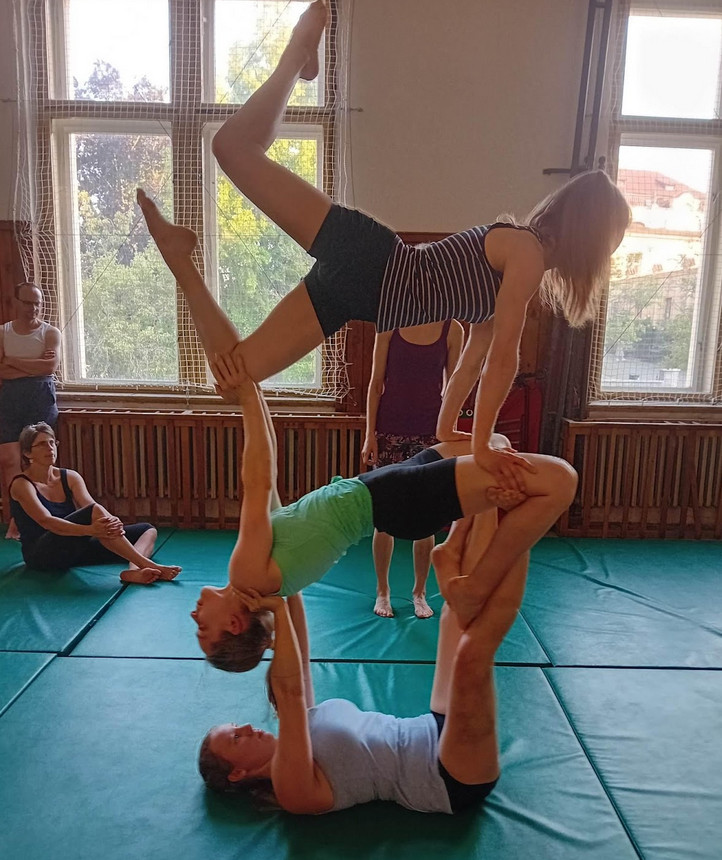
\includegraphics[width=0.9\linewidth]{./akrojoga-1.jpg}
\end{wrapfigure}

Akrojóga je zajímavá tím, že se cvičí v~páru, přičemž jeden ze dvojice, tzv. letec, létá vzduchem a cvičí na svém partnerovi, tzv. bázi, která většinou leží na zemi, popřípadě stojí. Oba dva řádně procvičí rovnováhu a koordinaci, zapojí celé tělo, zaposilují si i se protáhnou. Navíc je cvičení i o~důvěře v~druhého a o~vzájemné komunikaci. V~akrojóze letec cvičí jednotlivé samostatné prvky, které může následně jakkoli propojit a poskládat v~sestavu, tzv. flow. Flow může být krátké a jednoduché, nebo delší a složitější s~různými skoky do vzduchu, otočkami a stojkami.

Akrolekce jsou určené pro všechny zájemce jakékoli úrovně, fyzické zdatnosti, věku a pohlaví. První lekce proběhne v~pátek 20. září v~18–⁠⁠⁠⁠⁠⁠19:30 v~lodi hlavního sálu v~sokolovně. Pro členy sokola je lekce zdarma, pro nečleny je cena 100 Kč. S~sebou je potřeba jen sportovní oblečení.

V~případě dotazů můžete kontaktovat Markétu Kolářovou na čísle 736 762 307 či e-mailu marketa.kolarova@sokol-liben.cz.

Na všechny se těší

\signature{Anička a Markéta}{}

\vspace*{12pt}
\begin{center}
  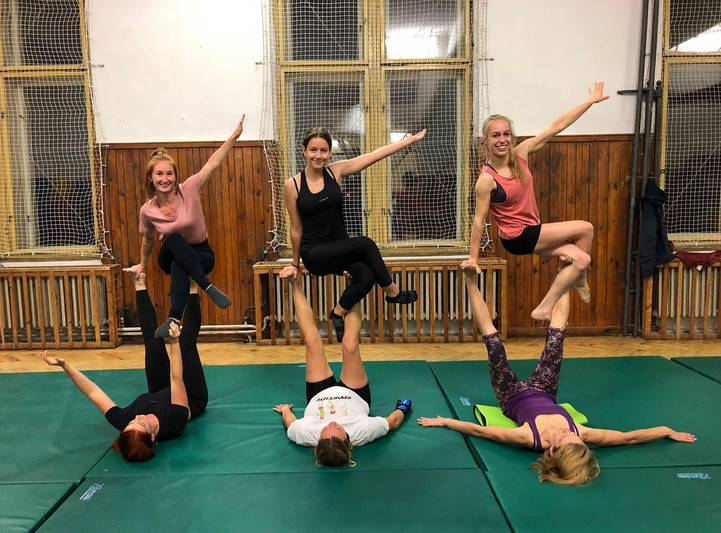
\includegraphics[width=0.8\linewidth]{./akrojoga-2.jpg}
\end{center}

\vspace*{24pt}

\post{Předškolní děti}
Do oddílu je zapsáno aktuálně skoro 90 děti. Tak velký počet si může dovolit jen díky cvičitelům a dobrovolníkům z~řad rodičů, kteří svůj volný čas věnují všestrannému sportovnímu rozvoji dětí.

Moc jim za to děkuji, protože bez nich by oddíl nemohl fungovat a připravovat děti na akce, které nás v~roce 2024 a 2025 čekají: závody v~míčovém trojboji, Akademie Sokola Libeň, gymnastické závody a atletické závody.

Děti začnou během října nacvičovat skladbu pro Akademii, takže už prosím nyní počítejte s~termínem 22. 11. od 16:00, kdy bude společný secvik dětí z~pondělní a čtvrteční hodiny.

A~pokud nevíte, co je to Akademie, tak si na webu České televize pusťte záznam sletu 2024. Jen se nás do toho sálu nevejdou tisíce, ale jen desítky.

Těším se na značkách.

\signature{Dana Cejpková}{vedoucí oddílu předškolních dětí}

\vspace*{24pt}

\post{Oddíl rodičů a dětí}
Oddíl má bohužel už od června plně vytíženou kapacitu. Jsou tedy desítky rodičů a dětí, kteří by rádi do Sokola chodili cvičit, ale my už pro ně bohužel nemáme místo.

Pokud je mezi vámi nadšenec, který by ve svém volném čase chtěl seznamovat rodiče a děti se základy všestrannosti, určitě se může přihlásit kterékoliv vedoucí cvičení a my mu vysvětlíme, co by to obnášelo. Jednota mu samozřejmě zajistí patřičná školení.

Během listopadové Akademie bude mít oddíl svoje vystoupení. Bude to na písničku… nechte se překvapit. :-)

Nácvik bude probíhat v~pondělních a čtvrtečních hodinách. Pokud chodíte cvičit v~úterý dopoledne, klidně přijďte na odpolední hodinu v~říjnu, kdy si budete moci vyzkoušet, zda by se Vám skladba líbila.

Těšíme se na Vás i Vaše děti na cvičení.

\signature{Jana, Dana a Jana}{cvičitelky rodičů a dětí}

\clearpage

\post{Informace o~oddílech žákyň a dorostenek}
Oddíly všestrannosti mladších a starších žákyň a dorostenek pokračují ve cvičení stejně jako v~minulém školním roce. V~letošním roce sice nebudou probíhat nácviky na slet, hned po prázdninách se ovšem budeme věnovat nácviku ukázek na listopadovou akademii.

I~tak se s~dívkami vrátíme k~"tradičnějšímu" uspořádání cvičebních hodin. Na programu bude zejména gymnastická průprava, cvičení na nářadích i akrobacie. Doplníme samozřejmě i hry a atletické disciplíny. Budeme cvičit hlavně uvnitř, protože vnitřní vybavení nabízí lepší možnosti pro pohybovou přípravu cvičenek. Cvičení pojímáme jako "nezávodní", rádi pomáháme holkám najít nebo upevnit vzájemná přátelství. Po prvních hodinách nás příjemně potěšilo, jak předškolní holky přecházejí do mladších žákyň a jak dřívější mladší žákyně pokračují ve cvičení v~oddíle starších žákyň. Holek do oddílů chodí dost, přesto se u~nás místa ještě najdou. Pokud byste tedy měli zájem přihlásit dívky do našich oddílů, ozvěte se vedoucím oddílů.
 
Mladší žákyně (mladší školní věk, orientačně 1.–⁠⁠⁠⁠⁠⁠4. třída) cvičí v~pondělí a čtvrtek od 17:00,
Starší žákyně a dorostenky (od 5. třídy výše) pak hned po nich –⁠⁠⁠⁠⁠⁠ v~pondělí a čtvrtek od 18:00.

Oddíl mladších žákyň vede Lenka Nováková, 602974524, novakovale@centrum.cz, oddíl starších žákyň vede s~Lenkou Květa Kerhartová, 734678455, kveta.kerhartova@sokol-liben.cz.

\signature{Lenka a Květa}{}
\vspace*{24pt}

\post{V~1. pololetí roku 2024 darovalo krev 141 sokolů}
Ve sletovém roce 2024 vstoupil projekt Sokolská kapka krve do jubilejního 10. ročníku. 
Za 1. pololetí roku 2024 své výsledky nahlásilo 18 jednot, kdy celkem 141 dárců absolvovalo 246 odběrů.
Průběžné 1. místo obhájil opět Sokol Komárov z~župy Jungmannovy, kde 35 dárců absolvovalo celkem 62 odběrů. V~Sokole Libeň 4 dárci darovali celkem 6x. Výsledky za pololetí jsou k~dispozici na webu a na nástěnkách. 

Na podporu projektu se i letos konal hromadný odběr v~Tyršově domě a pozimní se bude konat u~příležitosti Památného dne sokolstva. 

Veškeré informace o~projektu a plánovaných hromadných odběrech najdete na www.sokolskakapkakrve.cz. Všechny dotazy též rád zodpovím na e-mailu: vit.jakoubek@sokol-liben.cz. Nezapomeňte mi nahlásit počet odběrů za 2. pololetí (případně i za 1. pololetí, pokud jste zapomněli) do 31. 1. 2025.

\signature{Vít Jakoubek}{zdravotník jednoty a koordinátor projektu}
\vspace*{24pt}

\post{Se Sokolem do divadla}
Po letní pauze se opět vydáme do víru kulturního dění hned s~několika nabídkami, které jsou sice již po termínu přihlašování, ale v~rámci volných míst se mohu pokusit zajistit místa i pro nové zájemce.

Vzdělávací programy v~Rudolfinu pokračují i v~další sezóně. Pokud byste měli zájem o~návštěvu tohoto cyklu, napište mi individuálně nejpozději do 10. října 2024 na e-mail uvedený zde níže. V~sezóně 2024/2025 jsou opět v~plánu 3 vzdělávací koncerty, a to:

\renewcommand{\arraystretch}{1}
\begin{itemize}
  \setlength\itemsep{-3pt}
  \item Dvořákova Anglická z~vysoké – 4. 11. 2024
  \item Čtvero ročních dob z~Benátek a Buenos Aires – 12. 12. 2024
  \item Obrázky z~výstavy – 20. 3. 2025
\end{itemize}

Z~připravovaných návštěv stojí za pozornost i návštěva Divadla Spejbla a Hurvínka, kde 11. 10. 2024 shlédne 62 přihlášených zájemců představení „Jak Hurvínek prodává nevěstu“. Toto představení pro děti stravitelnou formou kombinuje hurvínkovský vtip s~nejznámějšími áriemi slavné české opery. Pokud byste se k~nám chtěli na poslední chvíli přidat, pište na e-mail zde níže nejpozději do 30. září 2024 – pokusím se zajistit vstupenky v~rámci dispozic sálu.

Vrcholem kulturních počinů letošního roku bude beze sporu vyhrazené slavnostní představení v~Žižkovském divadle Járy Cimrmana, které se bude konat 24. 11. 2024 v~rámci oslav 140 let Sokola Libeň. Stručně můžeme shrnout, že po „Českém nebi“ se zaprášilo! Kapacita divadla se členy Sokola Libeň a jejich nejbližšími rodinnými příslušníky naplnila během několika málo hodin. Takto bleskový zájem předčil veškerá naše očekávání. Zároveň mě mrzí, že divadlo není větší, abychom mohli uspokojit všechny zájemce. Věřme tedy, že se akce vydaří a že bude odrazovým můstkem pro podobné výjimečné akce do budoucna.

\signature{Miloslav Doupal}{e-mail: mila.doupal@sokol-liben.cz}
\vspace*{24pt}


\post{Pietní akt}
Nazdar, 

\noindent
ráda bych všechny členy a příznivce Sokola Libeň pozvala na pietní akt k~Památnému dni sokolstva, který proběhne ve čtvrtek 10. října od 18:00 do cca 20:00 ve vestibulu naší sokolovny. Kdo by měl zájem se zúčastnit jako krojovaný nebo mi chtěl pomoct s~organizací, neváhejte mi napsat (736 704 449).

Na všechny se těší
\signature{Bára Jeníková}{}

\begin{center}
  \noindent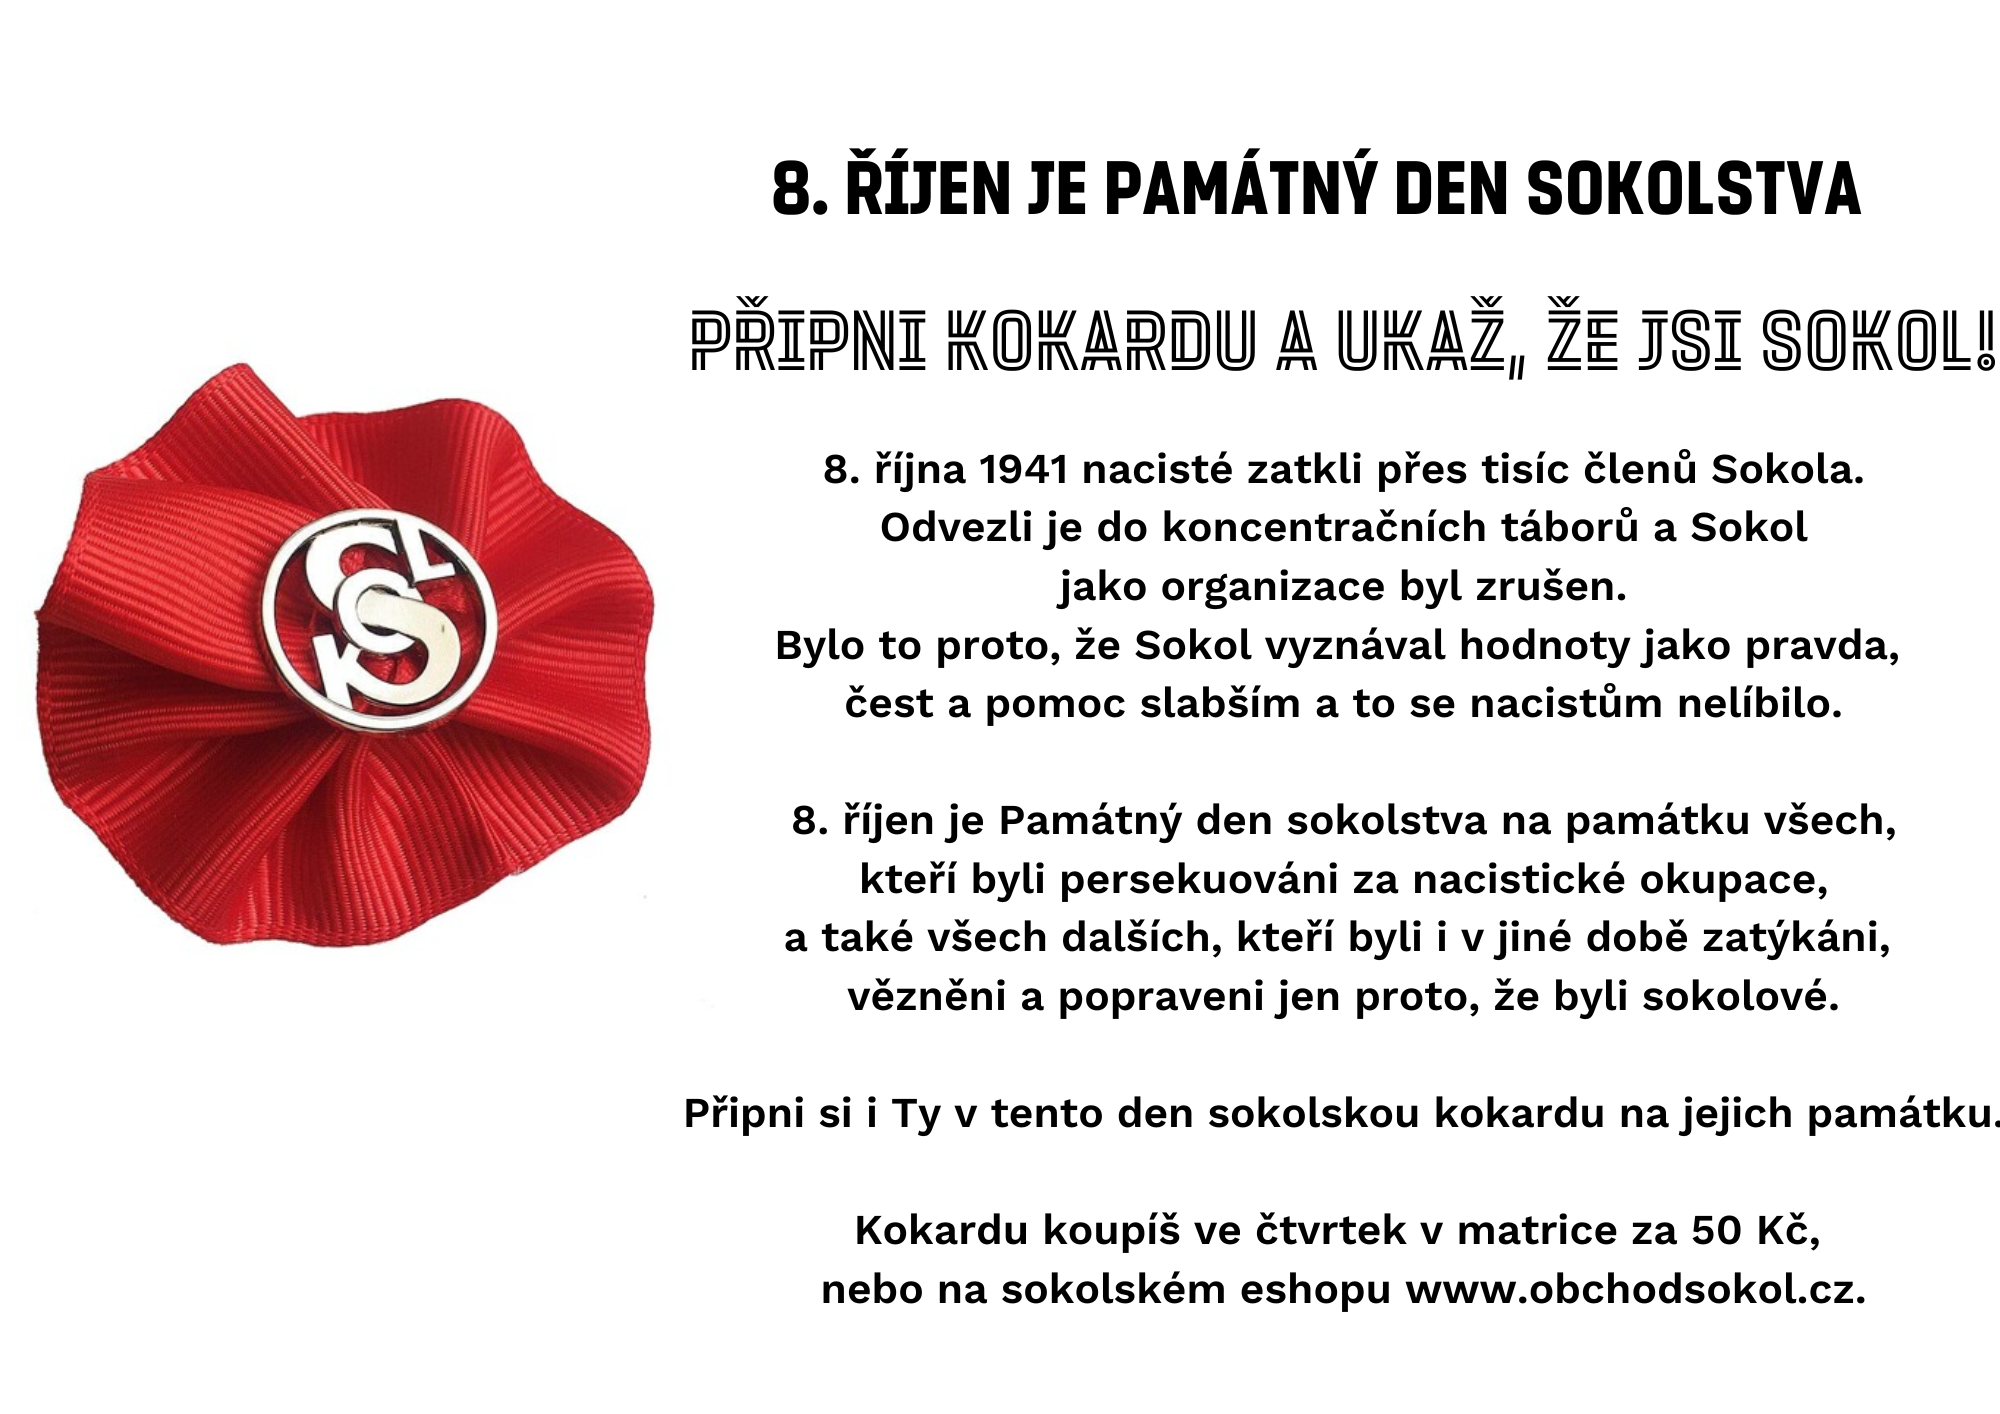
\includegraphics[width=\linewidth]{pripni-kokardu.png}
\end{center}


\post{Hledá se kmotra!}
Děkuji všem dárcům a přispěvatelům na nový prapor oddílu mužů.

Vybrali jsme víc peněz než bylo potřeba a podle slibu, šel výtěžek nad potřebnou částku na fungování sokolovny. Prapor je již ve výrobě a převezmu jej 21. září. Jednotě ho poté slavnostně předáme během podzimní Akademie, která bude 23. listopadu.

Aby předání splnilo všechny náležitosti, měl by mít prapor svoji kmotru. Pokud vás napadá, dobrá duše, která by byla ochotna kmotřit praporu při předání, dejte mi prosím vědět.

\signature{náčelník}{}

\vspace*{24pt}

\begin{center}
  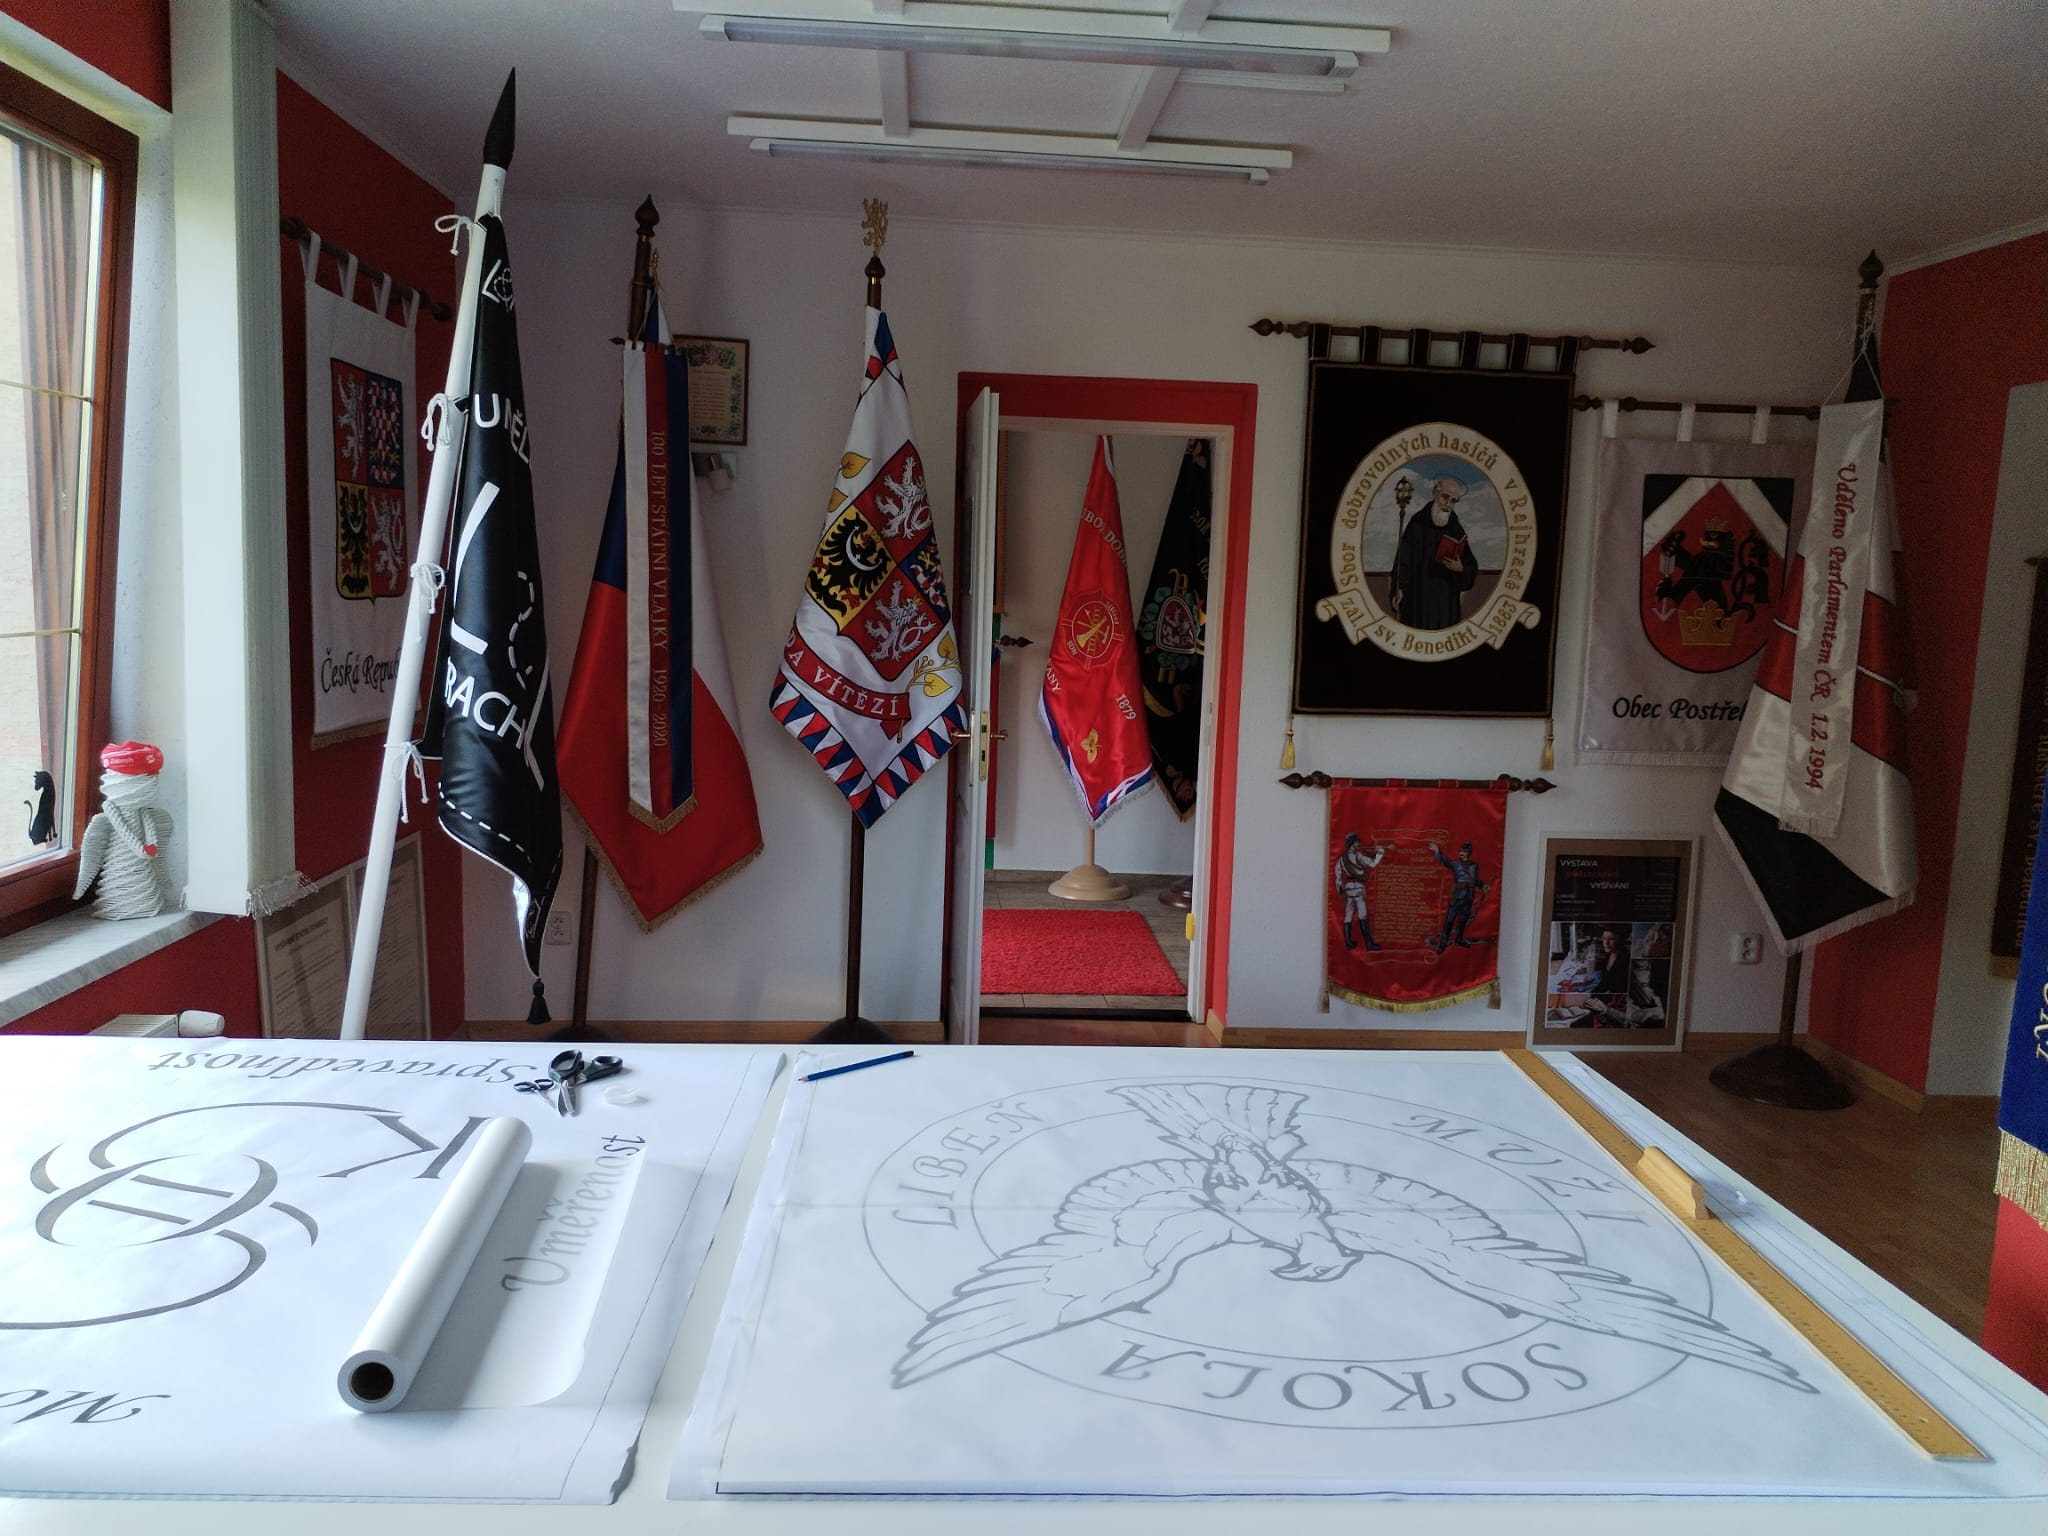
\includegraphics[width=\linewidth]{./prapor-2.jpg}
\end{center}

\clearpage

\post{Přetah lanem}
Měli jsme za sebou mistrovství přetahování lanem ve Všejanech a malou grilovačku, kde jsme si vyměnili dojmy a radili se, co budeme dělat dál.

Nadhodil jsem tam, že v~září bude mistrovství světa v~Mannheimu a že je to pravděpodobně na dlouho dobu poslední svěťák, kam se budeme moct podívat na vlastní náklady, protože ty další budou na Tchaj-wanu a v~Jižní Africe. Celé jsme to postavili tak, že pojedem tak jako tak, a že pokud nás bude málo, budeme se jenom dívat. To, jestli budeme tahat, záleželo na složení týmu. Buď nás muselo jet aspoň 9 kluků nebo aspoň 9 holek, případně 4 holky, 4 kluci + 2 náhradníci. Dál byla důležitá cena, světová federace v~přetahování lanem nabízí balíčky pro atlety, které zahrnují ubytování, jídlo, akreditaci a dopravu z~hotelu na stadion v~několika třídách luxusu, z~nichž nejlevnější stála €755, to pro nás bylo moc. Řekli jsme si, že se budeme připravovat, trénovat, hubnout a že zkusíme sehnat peníze nebo snížit náklady tím, že si seženeme bydlení a akreditaci si zaplatíme vedle. To byl konec června.

Tréninky neměly zdaleka ideální účast. Pro srovnání, ostatní týmy spolu tahají $3\times3$ hodiny týdně v~plné sestavě. My si sice přidali jeden trénink týdně navíc, účast byla vyšší než během roku bývá, ale všichni jsme se kvůli táborům a dovoleným sešli jen dvakrát. I~to bylo víc, než jsem čekal. Zaplatili jsme akreditace a startovné týmu (€125 na osobu a k~tomu €150 za tým), zvážili se a zjistili, že budeme moct tahat jen v~kategorii mix do 580\,kg (celkové váhy týmu). Já se váhově do sestavy nevešel a ani mě to příliš nemrzelo. Pořád jsem to bral tak, že jsme se měli jet původně jenom dívat. Nicméně pro případ střídání, nebo kdyby jinému týmu někdo vypadl, jsem se připravoval stejně jako ostatní. Plánovaná sestava byla:
\begin{center}
Dominik Absolon \\
Jonáš Čábelka \\
Petr Kříž \\
Jan Kerhart \\
Květa Kerhartová \\
Pavla Dvořáková \\
Adéla Šišková \\
Mery (Mariana) Majoberová \\
a Eva Šádková jako náhradnice
\end{center}

Potřebovali jsme dresy, abychom nedělali ostudu v~tričkách. Tahá se tradičně v~retro rugby dresech. Od Jacka ze Sokola jsme měli kontakt na Tonyho Brabce s~obchodem s~dresy hned u~vinohradské sokolovny, ten nám velkoryse půjčil pár dresů na zkoušku a pak jsme si plácli, že nám na ně vyšije sokolíky a vyztuží nám boky, aby lépe odolávaly lanu (tak to dresy mají). Vymysleli jsme si, že budem mít červené kraťasy (těch máme nejvíc) a že si seženeme kšiltovky, na které dáme kokardu s~perem.

\begin{wrapfigure}{l}{0.5\textwidth}
  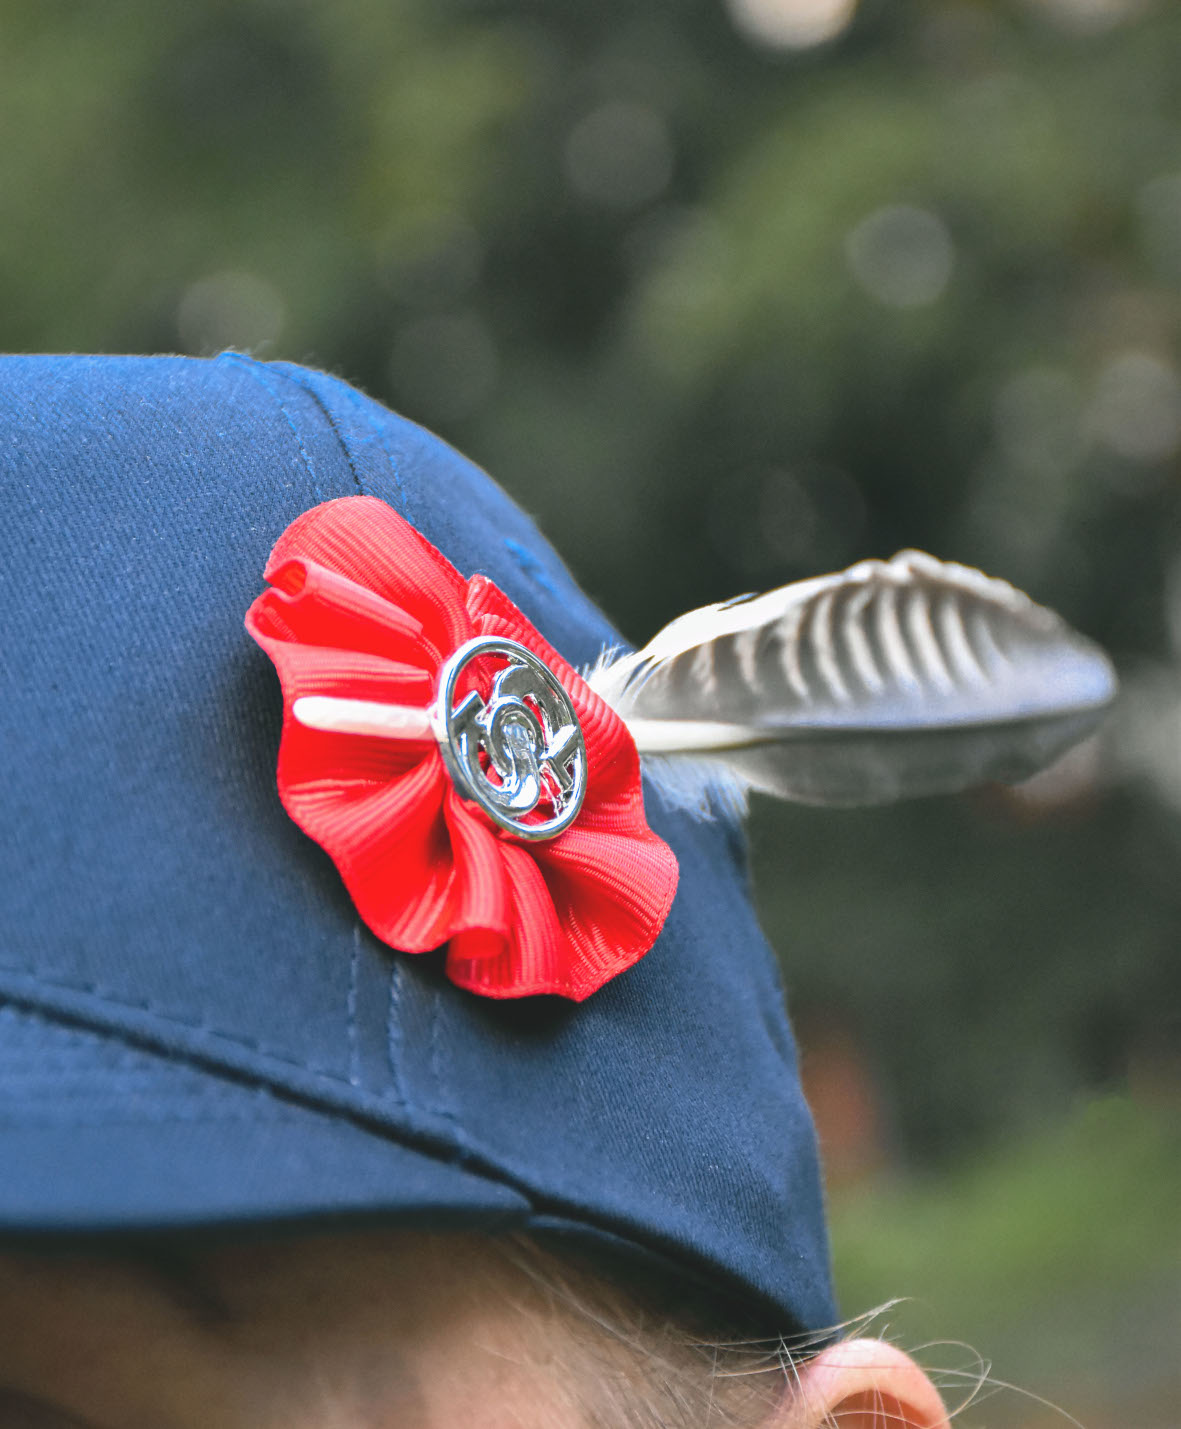
\includegraphics[width=0.9\linewidth]{./lano-kokarda.jpg}
\end{wrapfigure}

Turnaj se pomalu blížil, v~okolí Mannheimu jsme nesehnali ani sokolovnu, ani skautskou klubovnu k~přespání, tak nám náklady stouply o~cenu úplně nejlevnějšího ubytování, které jsme našli.

Datum odjezdu se blížil a přišla první infarktová situace, totiž že nebyly připraveny dresy. Tony je tedy vyzvedl na Moravě, kam pro ně jel na otočku, a předal nám je nevyšité s~tím, že v~nich odtaháme a necháme je došít po turnaji. Povedlo se mu je předat 20 minut před naším odjezdem.

V~úterý 3. září 2024 ve čtyři hodiny odpoledne jsme symbolicky zvedli kotvu (nejtěžšího člena týmu, jenž má kolem sebe uvázané lano na konci) a vyrazili dvěma auty do Mannheimu. Cestou jsme si zvedali náladu vtipy o~Lotyších, pro kontext je třeba vědět, že jsme tou dobou třetí den hladověli, abychom se vešli do váhového limitu. Pro ukázku humoru o~Lotyších vám dva zmíním.

\begin{center}
  \textit{Co dostanou děti v~Lotyšsku pod stromeček? Zemiaka. Ale to není zemiak. Je to kámen. Takový je život.}
\end{center}

\begin{center}
  \textit{Politbyro poslalo do gulagu balík na Vánoce. Každý chlap dostal kámen v~barvě zemiaka. Politbyro bylo v~tomto roce štědré. Loni poslali víc chlapů.}
\end{center}

Do hotelu jsme se dostali kolem půlnoci. Rozdělili jsme se do tří pokojů a pro kontrolu jsme se zvážili.
Výpočet nám vycházel tak, že jsme zhubli víc, než jsme čekali, a že pokud zhubneme do rána ještě 4,5 kg, mohli bychom se druhý den zeptat organizátorů, jestli by se bylo možné přihlásit i do kategorie mix (kluci holky) do 23 let pod 560 kg. Jediní dva třicátníci jsme si hodili nožky nahoru a hladili si hlad, dvacátníci na sebe nabalili mikiny a šli se proběhnout po Mannheimu. Okolo druhé ranní hodiny přiběhli a měli potřebnou váhu.

\noindent\textbf{4. září 2024}
\vspace*{6pt}

\begin{wrapfigure}{r}{0.5\textwidth}
  \vspace*{-\intextsep}
  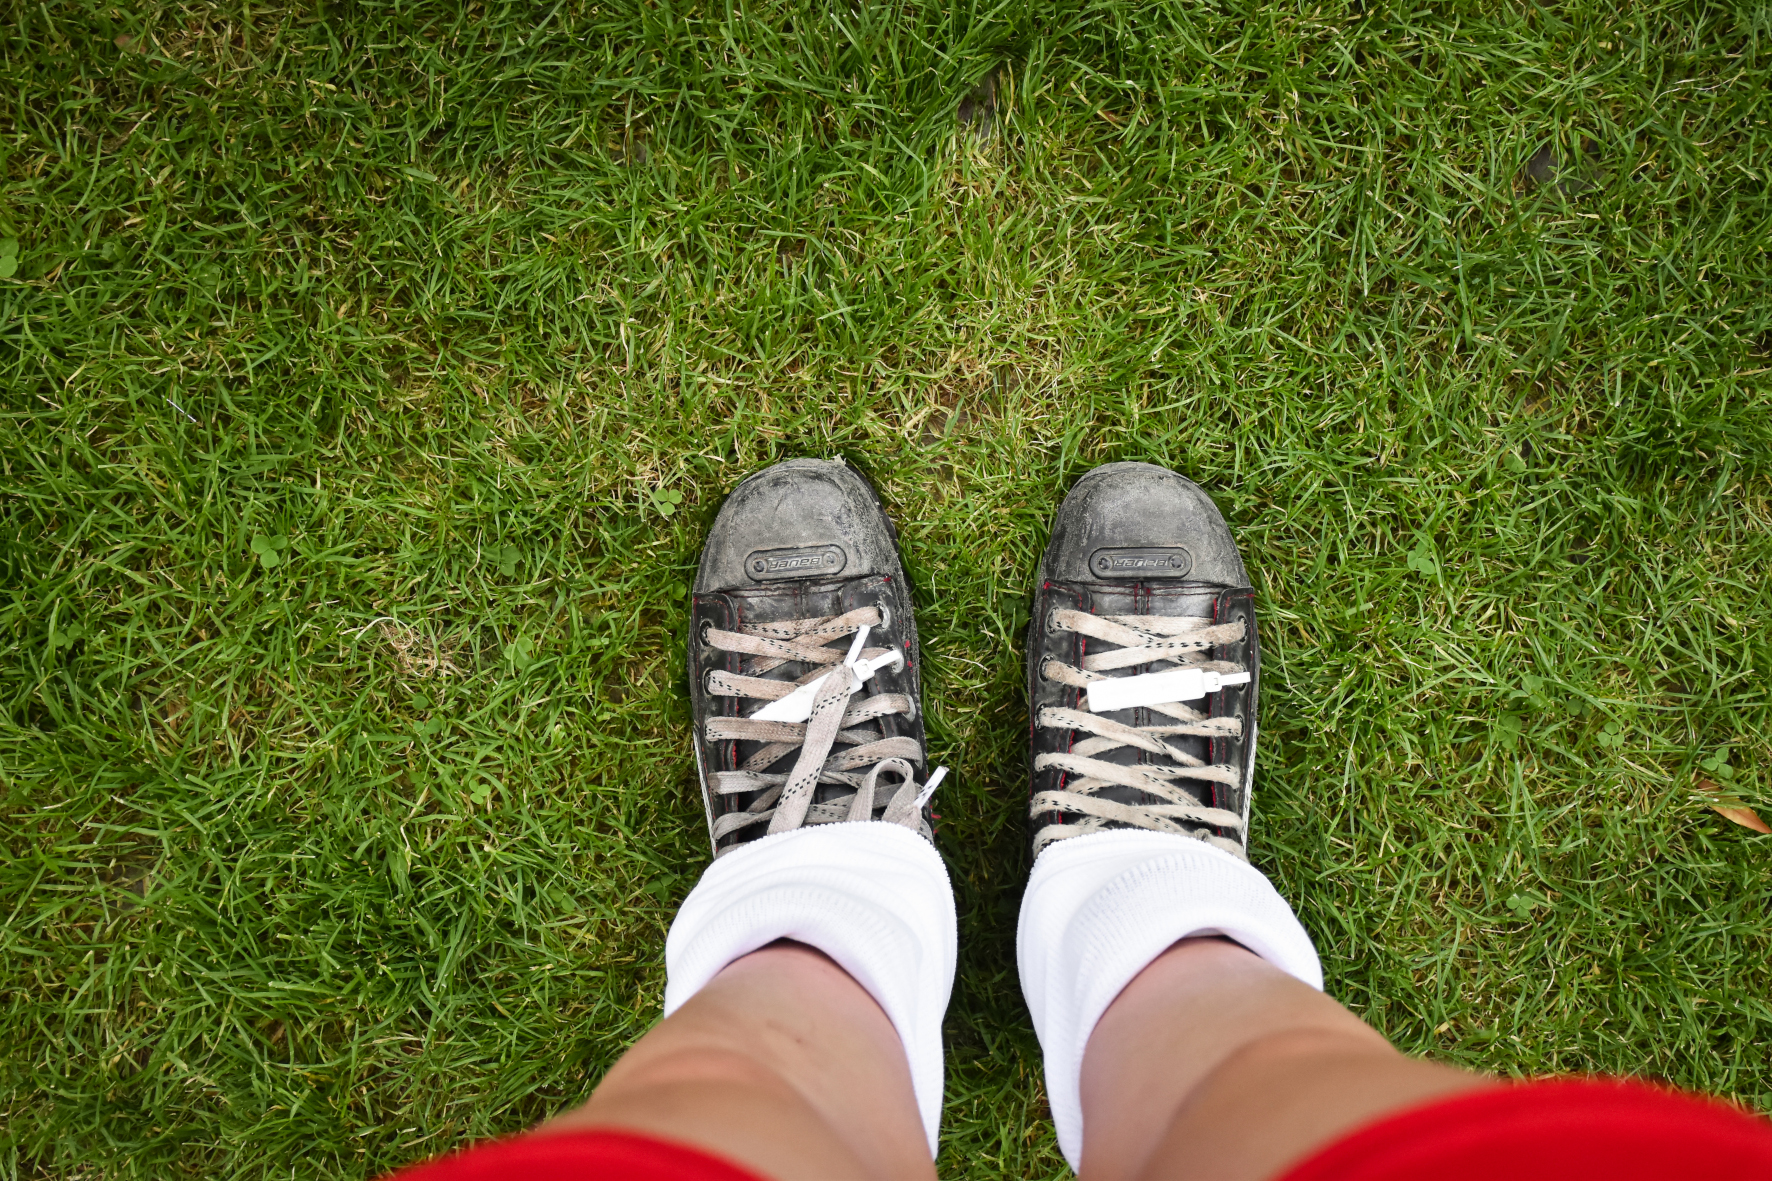
\includegraphics[width=0.9\linewidth]{./lano-boty.jpg}
\end{wrapfigure}

\noindent
K~snídani nebylo nic. Vyrazili jsme na půl osmou hodinu s~auty plnými tahaček (bot) ke stadionu, kde měl probíhat turnaj.

Zatímco jsem byl v~kanceláři a poznal ohromnou vstřícnost organizátorů (přihlásili nás do druhé kategorie), ostatní venku ve frontě na vážení stihla průtrž mračen. Mokří jsme se frontou dostali až k~vážení, kde jsme ztropili drobný skandál. Špatně jsem porozuměl pravidlům vážení, a tak jsme se šli vážit jen ve spodním prádle, v~pravidlech ale je, že je potřeba mít na sobě alespoň dvě vrstvy. Došlo tak k~tomu, že jsme si mezi sebou půjčovali jedny kraťasy pro toho, kdo šel zrovna na váhu.

Vážení dopadlo následovně:

\vspace*{6pt}
\noindent
\begin{tabular*}{\linewidth}[]{lrrr}
  & Váha v~červnu & Výsledná váha & Rozdíl \\
  \hline \\
  Jonáš Čábelka & 92 kg & 86,8 kg & 5,2 kg \\
  Dominik Absolon & 79 kg & 73,2 kg & 5,8 kg \\
  Jan Kerhart & 72 kg & 68,2 kg & 3,8 kg \\
  Petr Kříž & 67 kg & 61,7 kg & 5,3 kg \\
  Josef Kubišta & 78 kg & 72,4 kg & 5,6 kg \\
  Adéla Šišková & 67 kg & 64,6 kg & 2,4 kg \\
  Květa Kerhartová & 74 kg & 69,4 kg & 4,6 kg \\
  Pavla Dvořáková & 64 kg & 62,8 kg & 1,2 kg \\
  Mariana Majoberová & 71 kg & 66,8 kg & 4,2 kg \\
  Eva Šádková & 63 kg & 58,7 kg & 4,3 kg \\
\end{tabular*}
\vspace*{6pt}

Díky tomu, že jsme byli přihlášeni i do druhé kategorie a že jsme navážili méně, než jsem čekal, jsem se dostal do sestavy v~té těžší a nikoho nevyšachoval tak, aby si vůbec nezatahal.

Přišla chvíle se pozvolna najíst, napít a snažit se vybojovat váhu zpět, k~tomu ale nedošlo hned. Protože mám od přírody štěstí, že jsem při každé návštěvě letiště pozván na test na nebezpečné látky nebo nějakou kontrolu navíc, někdo si vyhodnotil, že bych mohl být na steroidech, a tak jsem byl pozván k~dopingové zkoušce ze vzorku krve. Byla to zajímavá a příjemná zkušenost. Dominik byl celou dobu se mnou, jako svědek, že nebyly výsledky zmanipulovány, a aby mě utěšoval.

Po zvážení jsme šli ke kontrole tahaček a vesty pro kotvu. Prošly nám všechny boty až na jeden pár, měl špatně usazený šroub na podrážce, tak byla nutná oprava. Tu jsme si nechali do hotelu, hlad byl silnější než touha po opravování.

Pája pro nás vybrala fajn kavárnu, kde jsme si řekli sestavu pro čtvrteční tahání v~kategorii MIX580, vysvětlili si, jak probíhá razítkování (stamping), a poté jsme se rozešli prohlédnout si město, nakoupit si zásoby a odpočinout si.

Ve frontě na kebab jsem zavolal reprezentačnímu trenérovi. Nabídl jsem mu jména našich tahounů a váhy, které jsme navážili, taky jsem mu nabídl k~dispozici nářadí a materiál k~opravě bot a boty samotné, protože jsme vzali do zásoby náhradní tahačky, pro všechny případy. Poměrně rychle mi řekl, že nic z~toho nepotřebuje a že děkuje, tak jsem mu už řekl jen, že máme v~Mannheimu kompletní tým U23MIX560, a že kdyby byla možnost, tak bychom rádi tahali v~reprezentaci v~neděli. Turnaj totiž probíhá tak, že první dva dny je mistrovství klubů, kde jsme byli jako Sokol, třetí a čtvrtý den je mistrovství světa, kde závodí národní týmy. Podle očekávání mi bylo řečeno, že uzávěrka národních týmů byla už dávno a že reprezentovat nemůžem, tím hovor skončil.

Několik minut poté mi volal předseda České unie v~přetahování lanem, došlo totiž k~nedorozumění, kdy si myslel, že jsem přihlásil někoho navíc, kdo nebyl registrován v~Národní sportovní agentuře do nové kategorie, kterou jsem předem nenahlásil. Celou situaci jsem vysvětlil a popsal i rozhovor s~reprezentačním trenérem. Předseda ale řekl, že se na možnost reprezentace zeptá, že je vedení TWIF (Tug of war federation) velice vstřícné a pružné. A~tak se stalo, že z~původního plánu jet se do Mannheimu podívat jen jako diváci a možná si zatahat v~jedné kategorii staly dvě kategorie za Sokol a juniorská kategorie v~reprezentačním dresu.

Po obědě jsme se na chvilku zastavili v~parku vedle hotelu na krátké focení v~dresech. Mery krásně fotí, a tak se s~vámi můžeme podělit o~to, jací jsme byli fešáci.

\begin{center}
  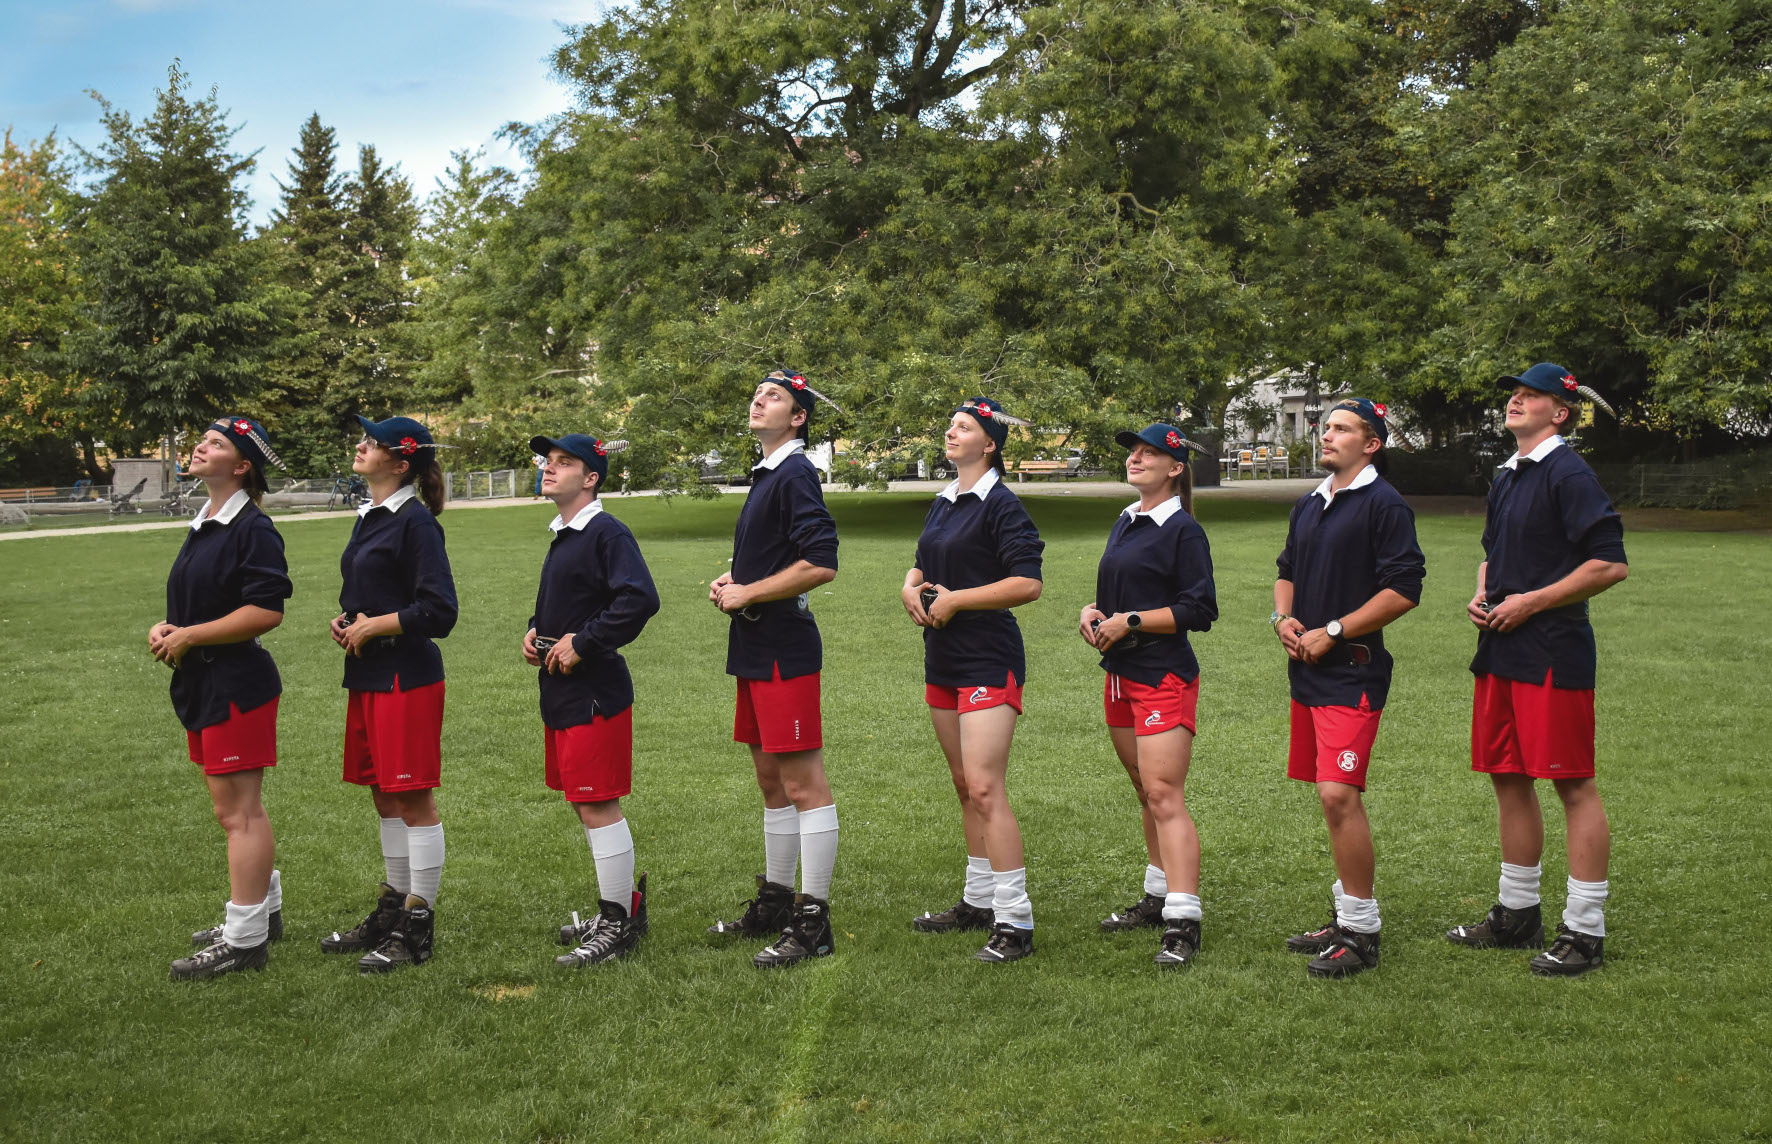
\includegraphics[width=\linewidth]{./lano-team.jpg}
\end{center}

Po focení jsme upravili stržený závit na nevyhovujících tahačkách a zjistili, že na stejném hotelu jako my jsou ubytovaní tahači z~klubu Atlants Kyjev. Popovídali jsme si, v~jakých kategoriích budeme soutěžit, dozvěděli se, že jejich klub tahá lano halově a že Mannheim bude jejich první zkušenost v~tahání na trávě. V~přetahování lanem se indoor a outdoor liší opravdu hodně. Taky říkali, že mají ještě několik neschválených bot, tak jsme vzali Táňu, Viktorii a Veroniku na stadion autem zkontrolovat si boty společně. Mimo kontroly bot jsme na místě ještě odevzdali soupisku pro nadcházející turnaje a potřebovali jsme si vyzvednout arch pro národní tým. Setkali jsme se s~Dominikem s~představitelkou TWIF Maaike Hornstra, která nás úplně zaskočila charismatem. Řekl jsem, že jsem Josef, a Maaike na to, že to ví. Že jsme ze Sokola z~Prahy a že jsme se chtěli dodatečně přihlásit do U23MIX560 a do národního týmu a že nás tam už zapsala. Že mi to psala whatsappem, který jsme zjistili, že mi nechodí, a hned to opravili. Taky se ujistila, že dorazíme s~Dominikem večer na informační schůzku zástupců klubů. To jsme v~plánu měli.

Dál jsme vysadili Ukrajinky na hotelu a udělali si krátkou poradu ohledně pravidel. Vysvětlili si jejich signalizaci, čeho se vyvarovat a jak bude turnaj probíhat.

Ve 21\,h jsme se s~Dominikem dostavili do kongresového sálu na schůzku k~turnaji. Bylo nám upřímně trochu stydno, zatímco ostatní zástupci svých zemí byli v~čínských hedvábných krojích, Ukrajinci v~krásných vyšívankách a každý měl alespoň reprezentační mikinu, my byli v~sokolských tričkách propocených po celém dni. Říkali jsme si, že by to byla zrovna vhodná příležitost pro sokolský společenský oděv, který nám zatím nedorazil. K~tomu jsme byli dotázáni na drobnou nesrovnalost z~české strany ohledně členství ve federaci. Naštěstí byli organizátoři mimořádně přívětiví a plní pochopení. S~důležitými informacemi jsme dorazili na hotel před jedenáctou hodinou a stručně o~nich spravili ostatní. Dohodli jsme se na budíčku, na tom, kdo pojede na stadion autem s~tahačkama a kdo městskou dopravou, a šli spát před velkým dnem.


\vspace*{12pt}
\noindent\textbf{Čtvrtek 5. září – první den turnaje Club open}
\vspace*{6pt}

\noindent
Na stadion jsme dorazili na devátou hodinu, kdy začínal dopolední program, ten náš měl začít v~jednu a byl posunut na druhou hodinu. Stamping nám začal až ve dvanáct hodin. Měli jsme tedy 3 hodiny na sledování zápasů a na jejich průběh. Naše tepláková liga bez řádných pravidel z~louky na Rohanu ani koukání na youtube nemohla připravit naše nováčky na to, jak tah vypadá doopravdy. A~tak bylo na co koukat, jak na rychlost a podobu startovních povelů, tak na řazení, kdy a kde máme být, ustrojení kotevníků a podobně. Koukat bylo opravdu na co.

Ve dvanáct hodin jsme se dostavili už převlečeni v~dresech ke stampingu. Ten spočívá v~identifikaci tahounů, kontrole se soupiskou a označení razítkem s~kódem kategorie. Jedno razítko fasujeme na levé stehno, druhé na levé předloktí. Označeni jsme si našli volný stan v~zóně pro atlety, každý tým si tam může zabrat stan, který chce, a vyzdobit nebo vytunit si ho podle svého. Krom vlajek a symbolů klubů to byla často masážní lehátka, basy s~vodou, lékárničky, repráky s~hudbou a podobně. Naší stáji dominoval binec a sokolík Pepík, na kterého jsme tentokrát zapomínali víc, než kdy dřív.

Dopolední program se opravdu protáhl. Navíc, jak jsme se těšili, způsobili jsme si zmatky v~komunikaci, a tak si většina z~nás namazala ruce pryskyřicí už ve dvě hodiny a s~ulepenýma rukama jsme čekali ve vedru, než na nás přijde řada.

Na laně jsme byli v~sestavě odpředu:

\vspace*{6pt}

Květa Kerhartová

Jan Kerhart

Adéla Šišková

Pavla Dvořáková

Dominik Absolon

Josef Kubišta

Mery Majoberová

a Jonáš Čábelka jako kotevník

\vspace*{6pt}

Eva Šádková jako vodonoška

Petr Kříž jako kouč

\vspace*{6pt}

Tradice při zápasech v~přetahování lanem je, že si před tahem kouči vymění drobný dárek. Ve spolupráci s~Jirkou Braným, náčelníkem Sokola Praha VII, jsme si připravili špachtle s~vylaserovaným sokolem z~poštovní známky Alfonse Muchy a nápisem Sokol Tug of war v~sokolském fontu. Špachtle se používá k~čištění bot od bláta mezi tahy.

První klub, proti kterému jsme nastoupili, byl Ažuolas z~Litvy. První tah trval 1\,min 19\,s, druhý 1\,min 2\,s, oba jsme prohráli a vysloužili si jeden trestný bod. Tím jsme se zapsali jako první start klubu Sokol na mezinárodní soutěži. Zároveň si Květa strhla hned v~prvním tahu kůži na dlani, kde se obvykle trhá na hrazdě.

Na celý turnaj jsme se už od samého začátku chystali s~tím, že pravděpodobně všechny tahy prohrajeme. Chystali jsme se co nejlíp, abychom dělali co nejméně chyb a náš tah vypadal co nejlépe. Jenže hned třetím tahem jsme očekávání předčili.

Druhý klub, se kterým jsme tahali, byl DJ's z~USA.
První tah trval 58\,s~a my vyhráli. Druhý trval 1\,min 33\,s, Američané nás nepřetáhli, ale my dostali 3 trestné body a vyfaulovali se (celkem jsme dostali 4 v~obou tazích). Dostali jsme tedy jeden bod a snad vám nezkazím zážitek z~dalšího čtení, když vám prozradím, že to byl až do konce turnaje také bod poslední.

Třetí klub byl Brunnsberg ze Švédska. V~prvním 55\,s~dlouhém tahu si nás Švédi vyzkoušeli a ve druhém nás během 29\,s~přejeli jak válec. Trestný bod jsme nestihli dostat.

Čtvrtý souboj byl proti klubu Mutriku z~Baskicka. První tah trval 1\,min 3\,s, druhý 31\,s~a prohráli jsme oba s~čistým štítem.

Poslední trochu fiktivní klub se jmenoval Eschbachtal, šlo o~německý reprezentační tým, který se v~barvách Eschbachtalu rozcvičoval na sobotní mistrovství světa. V~jeho řadách byli naši kamarádi z~klubu Tauziehclub Allgäu Power Zell, u~kterých jsme byli už dvakrát na soustředění a z~jejichž rad a tipů stavíme naše tréninky. Na pozici 2 zepředu lana tahala Julia Freiß, která nám pomohla při návštěvě Prahy na podzimní brigádě v~sokolovně.

\begin{center}
  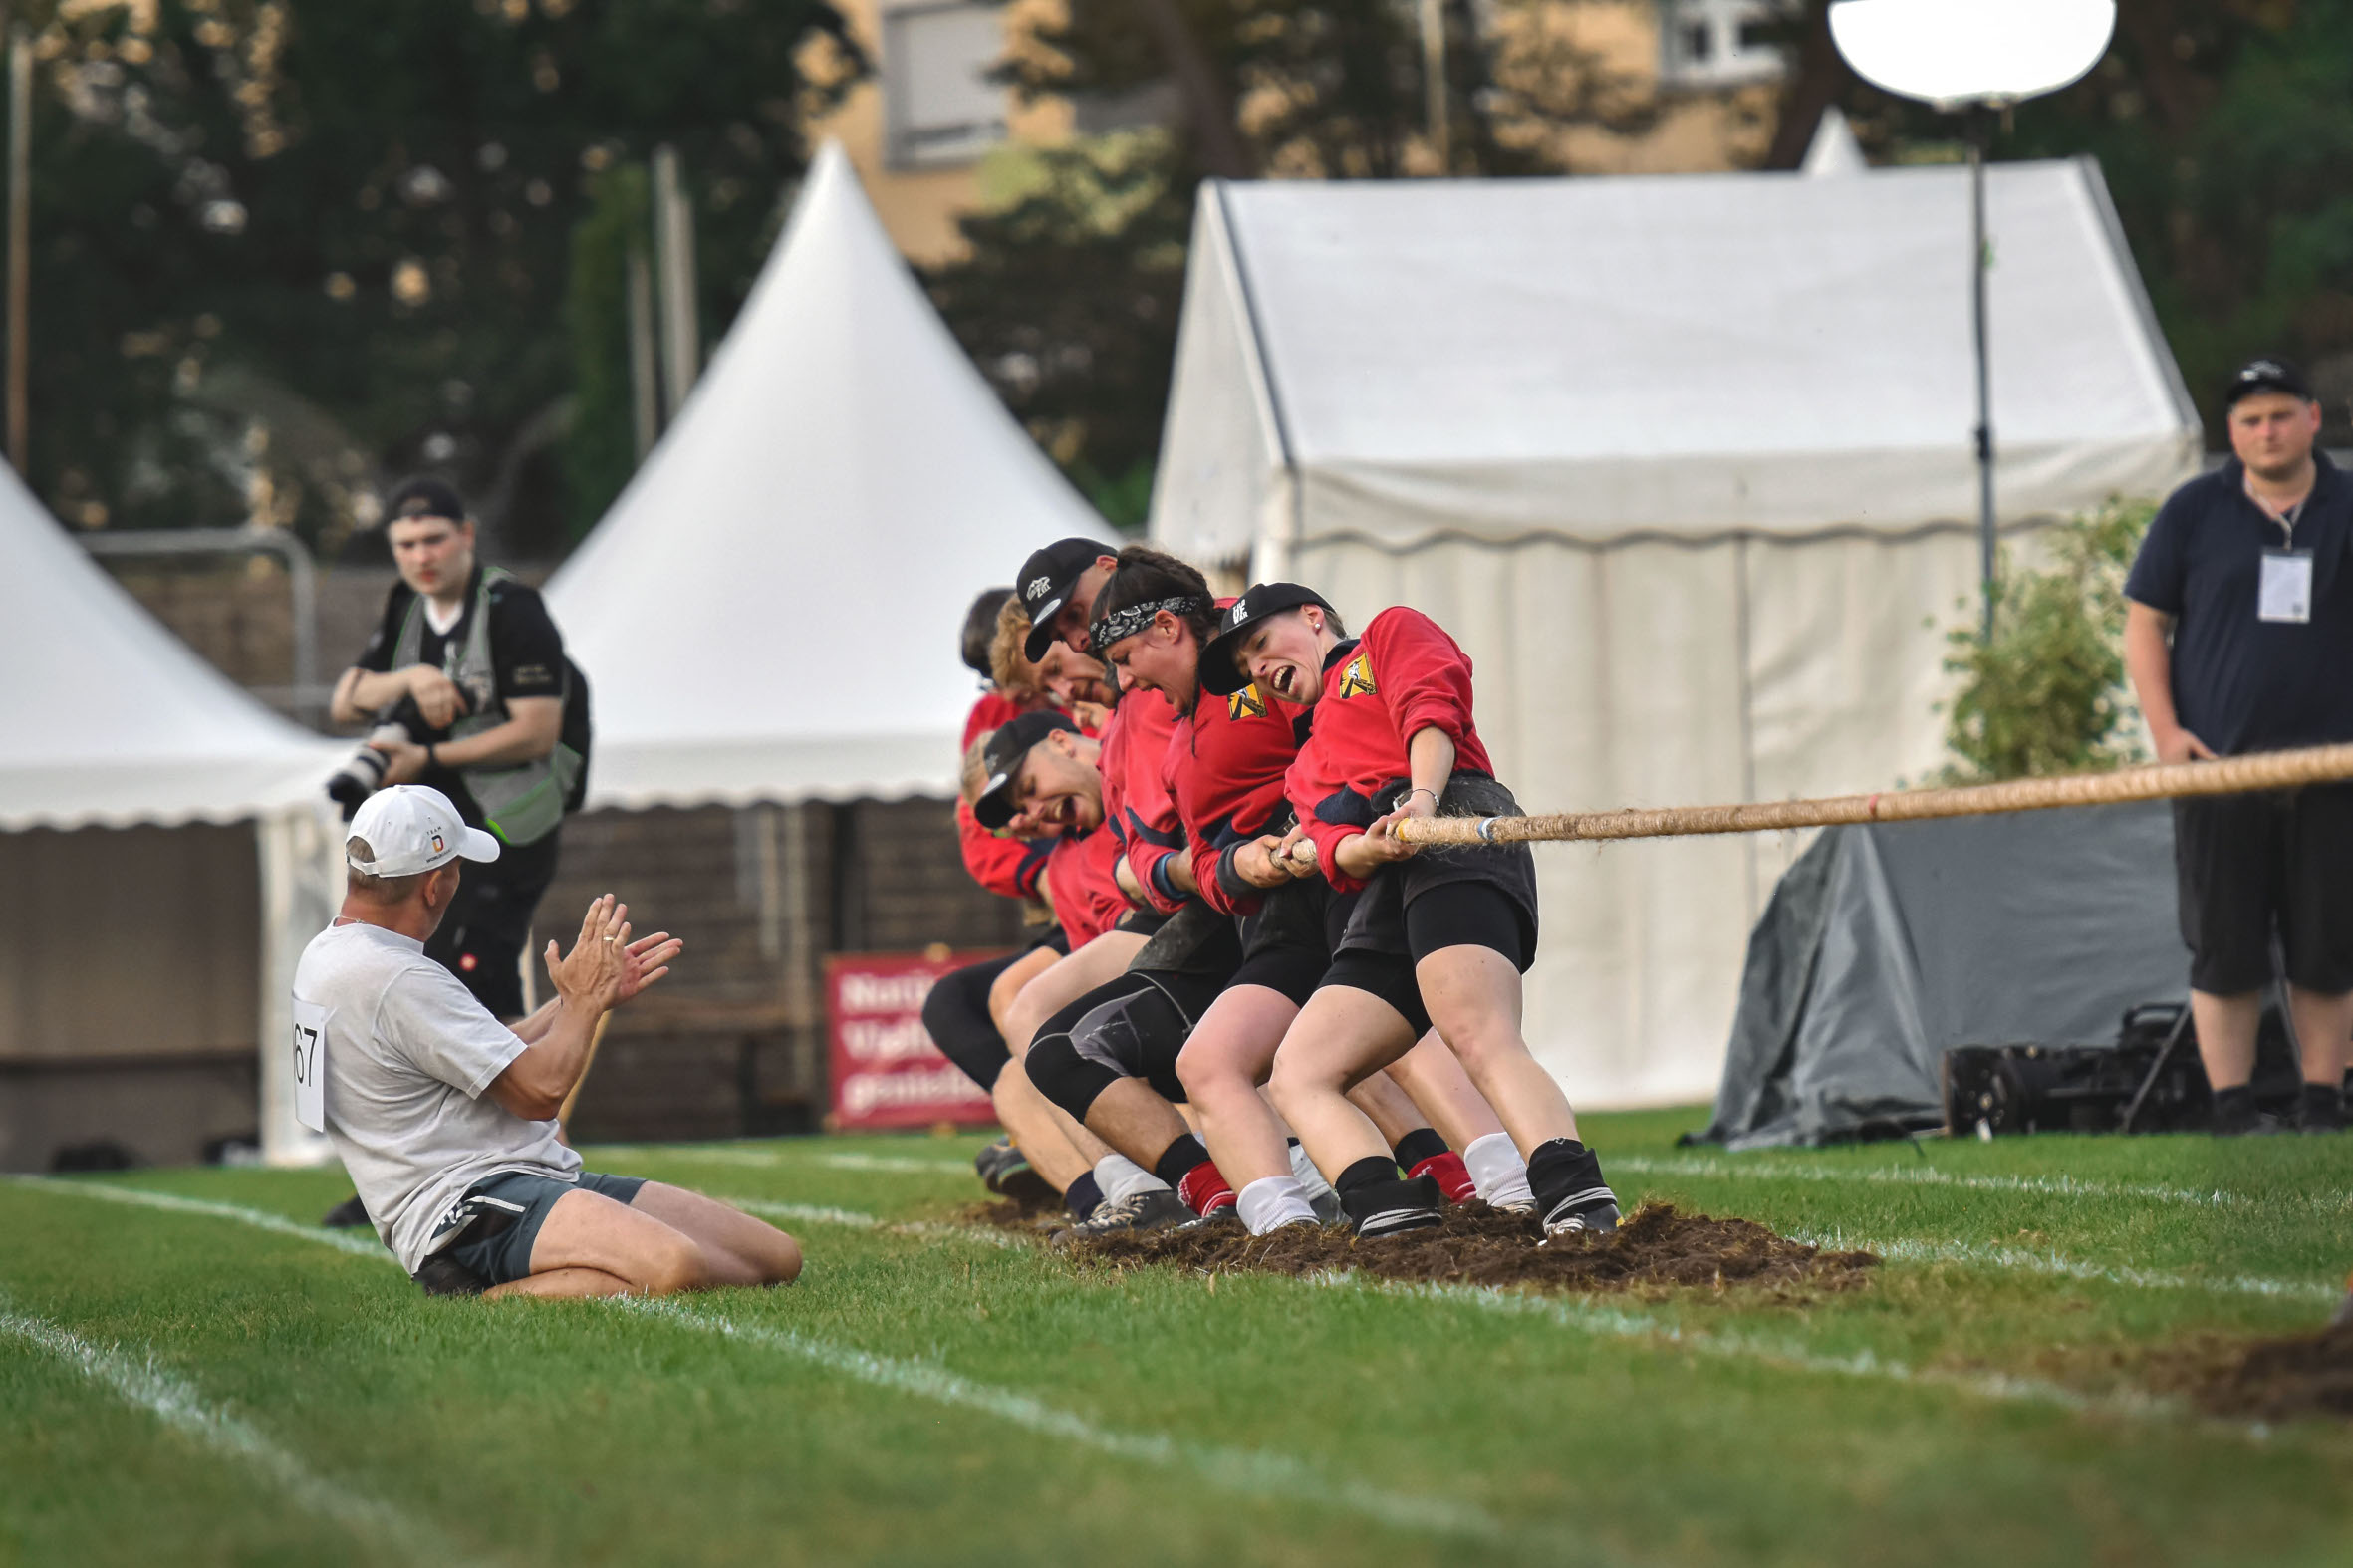
\includegraphics[width=\linewidth]{./lano-de.jpg}
\end{center}

Eschbachtal nás sfouknul v~prvním tahu za 32\,s, v~druhém jsme jim vzdorovali celých 40\,s. A~zvládli jsme se opět sklouznout bez trestného bodu. Nejen že nás sfouknul, ale vyhrál celý turnaj. My skončili z~celkem 27 klubů na posledním místě.

Turnaj jsme dokoukali až do konce a po deváté hodině a medailovém ceremoniálu jsme se vrátili na hotel a ještě si nějakou dobu povídali o~prvních zážitcích. Podívali se na videa našich tahů, řekli si, co všechno musí být lepší zítra, a zahráli si partičku Bangu.

Při gratulaci Eschbachtalu jsme se dozvěděli, že i když vyhráli všechny tahy naprosto suverénně, seděli ještě nad videoanalýzou do jedné ráno. A~protože jsou to kamarádi, poradili nejlepší těm nejhorším, na co na videích koukají a co pilují, i když je jejich tah zdánlivě nejlepší.

\vspace*{12pt}
\noindent\textbf{Pátek 6. září – druhý den turnaje Club open}
\vspace*{6pt}

\noindent
V~klidu jsme se vyspali, posnídali a vyrazili na stadion až chvíli po deváté hodině. Než došlo na stamping, stihli jsme se skamarádit s~dvěma holkama z~Baskicka a s~Litevci, vyměnili jsme si kontakty, ptali se, jestli je možné zúčastnit se jejich turnajů a kde se o~jejich konání dozvíme. Ptali jsme se, jak dlouho tahají a podobně.

Stamping byl stejně jako den předem ve 12 h. Sestavu na laně jsme oproti tréninkům upravili podle rad Němců. Sice měla daleko k~ideálu, ale přesuny nám zafungovaly a souhra a výška lana mezi tahouny za sebou nám sedla. Dál jsme v~turnaji neměnili rozestavění vůbec, dohodli jsme se, že se radši sehrajem tak, jak na laně jsme, než se přehazovat.

Sestava pro kategorii U23MIX560 byla odpředu na laně:

\vspace*{6pt}
Květa Kerhartová

Jan Kerhart

Eva Šádková

Adéla Šišková

Dominik Absolon

Mery Majoberová

Petr Kříž

a Jonáš Čábelka jako kotevník

\vspace*{6pt}

Pavla Dvořáková jako vodonoška

Josef Kubišta jako kouč

\vspace*{6pt}

První zápas byl proti týmu s~názvem England under 23\,s. První tah 48\,s, druhý 37\,s, oba jsme prohráli bez trestného bodu.

Druhý zápas byl proti klubu Goiherri z~Baskicka. První tah trval 2\,min 13\,s! Pokud jste při čtení sledovali pozorně časy našich tahů, můžete si všimnout zlepšení. Druhý tah trval 1\,min a 6\,s. Oba jsme prohráli bez trestného bodu.

Naši naději zchladil skotský klub Ayrshire. První tah trval 14\,s, druhý 40\,s~bez trestných bodů.

Další byl Het Loggertje z~Holandska. Tento klub měl zraněnou slečnu, a tak tahali v~sedmi, proto jsme na první tah nechali odpočinout Evě a na druhý tah Květě. První tah trval 19\,s, druhý 55\,s~bez trestných bodů. Byl to pro nás po Goiherri druhý hratelný tým, jen jsme na něj tentokrát neměli.

Předposlední klub byl opět z~Anglie a jmenoval se Killroe. První tah jsme bojovali 2\,min 44\,s, čímž jsme si zvedli osobák v~pobytu na laně, a druhý 44\,s, opět bez trestných bodů. Tou dobou měli kůži z~dlaní a prstů strhanou už i Kerhy a Áďa, což tah lehce znepříjemňovalo, nikdo se ale nevzdal a lano nepustil.

Poslední soupeř byl klub Valsbaai z~Jižní Afriky. V~tu dobu na náš poslední tah už byla na stadionu česká reprezentace, a tak jsme slyšeli hlasité povzbuzení, které opravdu pomohlo. První tah 20\,s, druhý jsme se zakousli na 1\,min 37\,s, bez trestných bodů.

V~průběhu turnaje docházelo k~drobným úpravám techniky a většinou nám fungovaly. Naprosto jsme se vyvarovali základních chyb, se kterými jsem tak nějak počítal a k~překvapení se neděly. I~tak děláme chyb stovky a do budoucna je budeme odstraňovat.

Krom strhaných dlaní, několika slziček a smutku, které jsme díky dobré náladě v~kabině rychle překonali, jsme měli ještě jednu nepříjemnost. Naše výprava totiž neměla dostatečně chránící vestu pro kotevníka. Tomu se lano dostalo na žebra a pohmoždilo mu je i se zády tak, že jsme využili možnosti fyzioterapeutického stanu. Zkušený borec si při pohledu na Jonáše posunul brýle na nose, pak ho hodinu lámal na lehátku a německy prohlásil, že bude žít. Měli jsme jeden den na regeneraci, než nastoupíme v~národních barvách. Mimo to ještě zakopl na schodech stadionu Dominik. Pád vypadal ošklivě, ale zranění byla jen lehká. Zranění jsme si nemohli dovolit, neměli jsme nikoho na střídání.

Po turnaji se konalo zahájení mistrovství světa a nástup vlajkonošů výprav. Tam už byla připravena česká reprezentace, která dorazila chvíli před tím.

Večer jsme si koupili na hotel pizzu a podělili se o~dojmy. Každý jsme řekli, co jsme měli na srdci, což bylo moc fajn. Úkol na sobotu byl odpočinout si, dát se do kupy, fandit českému nároďáku v~kategorii MIX580 a vyzvednout si reprezentační dresy na neděli.


\vspace*{12pt}
\noindent\textbf{Sobota 7. září – první den mistrovství světa}
\vspace*{6pt}

\noindent
Budíček tentokrát nebyl. Dohodli jsme se, že na stadion dorazíme až ve dvě hodiny, kdy měl začínat odpolední program a kategorie s~českou účastí.

Jediné, co jsme krom odpočinku dopoledne stihli, byl aktivní odpočinek. Pája jako vystudovaná magistra na FTVS si nás vzala na hodinu do parku, kde jsme procvičili namožené partie, malinko vykompenzovali posílení z~předešlých dvou dnů a obohatili si svojí zastaralou sokolskou rozcvičku o~soudobé cviky.
Patří se říci, že z~týmů, které jsme viděli, jsme se rozcvičovali před taháním jediní. Před každým tahem bylo k~dispozici vedle stadionu lano na roztahání, je tedy běžné vzít do ruky lano a rovnou jít tahat.

Abych čtenáře neunavoval příliš, přidám do přílohy odkaz na tabulku s~tahy české reprezentace. Podrobné informace budu psát jen o~sokolském týmu. Český výběr vybojoval tři body (dva vítězné tahy) proti Indii. Nejvyrovnanější a nejdelší tahy byly proti Srbsku, bohužel bez bodu.

Na konec turnaje byly rozstřelovací zápasy o~umístění. Českému výběru se ale ten proti USA v~podobném složení, v~jakém jsme je vyzvali my, bohužel porazit nepovedlo a skončili na celkovém 16. místě z~18 před Indií a Čínou.

Celý den bylo vedro, jak reportér TOW Jamie napsal na facebook \luv{}Hot as in devil's bakery\ruv{}, tak jsme se rozdělili na dvě party. Jedna počkala, až dotahá reprezentace, aby nám předala svoje dresy, druhá šla domů připravit večeři, při které se povedlo spustit požární poplach v~hotelu. To přispělo k~už tak dobré náladě v~týmu.

Dresy jsme dostali domů až poměrně pozdě večer, a tak jsme je místo praní jen rozvěsili k~uschnutí.


\vspace*{12pt}
\noindent\textbf{neděle 8. září – druhý den mistrovství světa}
\vspace*{6pt}

\noindent
Sestava pro kategorii U23MIX560 byla odpředu na laně stejná jako dva dny předtím:

\vspace*{6pt}
Květa Kerhartová

Jan Kerhart

Eva Šádková

Adéla Šišková

Dominik Absolon

Mery Majoberová

Petr Kříž

a Jonáš Čábelka jako kotevník

\vspace*{6pt}

Pavla Dvořáková jako vodonoška

Josef Kubišta jako kouč

\vspace*{6pt}

Zásadní změny oproti předchozím dnům byly dvě. Vydatně pršelo, a tak byl tahací povrch úplně jiný než dosud. A~Němci nám půjčili vestu pro kotvu, která byla výrazně jinak šitá než ta naše a hodně pomohla Jonášovi uchránit žebra, ale i víc zabrat.

Hned jako prvního soupeře jsme dostali čínskou Taipei, nejtěžšího soupeře, Tchaj-wan má svoji mladou základnu. První tah trval 43\,s, druhý 31\,s, trestný bod jsme nestihli.

Druhou jsme dostali Anglii. První tah trval 54\,s, druhý 1\,min 20\,s, opět bez trestného bodu.

Jako třetí jedny z~favoritů po boku Tchaj-wanu, a to Švýcary, a proti nim se nám povedl majstrštyk. První tah trval 47\,s, ale ten druhý 2\,min a 1\,s~a k~tomu bez trestného bodu, něco takového jsme proti Švýcarům opravdu nečekali a tah nespočíval jen v~zoufalé snaze co nejdéle se bránit, ale se Švýcary jsme i krůček popošli. Není prohra jako prohra, za tuhle jsme se opravdu stydět nemuseli.

Další na řadě byli Němci, ti si nás namazali na chleba. V~prvním tahu za 1\,min 17\,s, v~druhém za 41\,s, bez trestného bodu.

Zápas s~Baskickem patřil mezi nejlepší výkony, které jsme na turnaji předvedli. V~prvním tahu (1\,min 54\,s) jsme s~Basky ušli vzad celých pět kroků, než nás vzali, a špatný nebyl ani druhý tah 1\,min 7\,s. Ani v~zápase na naše poměry tak dlouhém jsme nedostali jediný trestný bod.

A~že už jsme se dostali na provozní teplotu, jsme dokázali délkou tahů i proti Jihoafrické republice. První tah 2\,min 4\,s, druhý 1\,min 14\,s, s~jedním trestným bodem.

Jako posledního soupeře turnaje jsme měli Skotsko, bylo vidět, že už taháme z~posledních sil. 45\,s~a 52\,s s~jedním trestným bodem a byl konec.

Mezi opravdu těžkými soupeři jsme si vysloužili poslední 8. místo. Po turnaji došlo k~výměně dresů a našich čepic. Dominik dostal reprezentační dres od Taipei, Pája zase od USA. K~tomu se povedlo vyhandlovat dvě mikiny USA Tug of war.

Bohužel se nám nepovedlo uzpůsobit si program abychom se mohli zúčastnit závěrečného večírku a museli jsme domů za školou a prací. Je to velká škoda, protože právě tam už mají všichni tahouni čas se bavit a nemusí se soustředit na nadcházející výkony. Takže jsme jen dokoukali finálové tahy kolem osmé hodiny večer, zabalili si a se zastávkou na večeři jsme jeli rovnou do Prahy, kde jsme v~pondělí okolo páté hodiny ranní vyložili auto v~sokolovně, vyfotili se na konci naší pouti a rozvezli se domů.

\begin{center}
  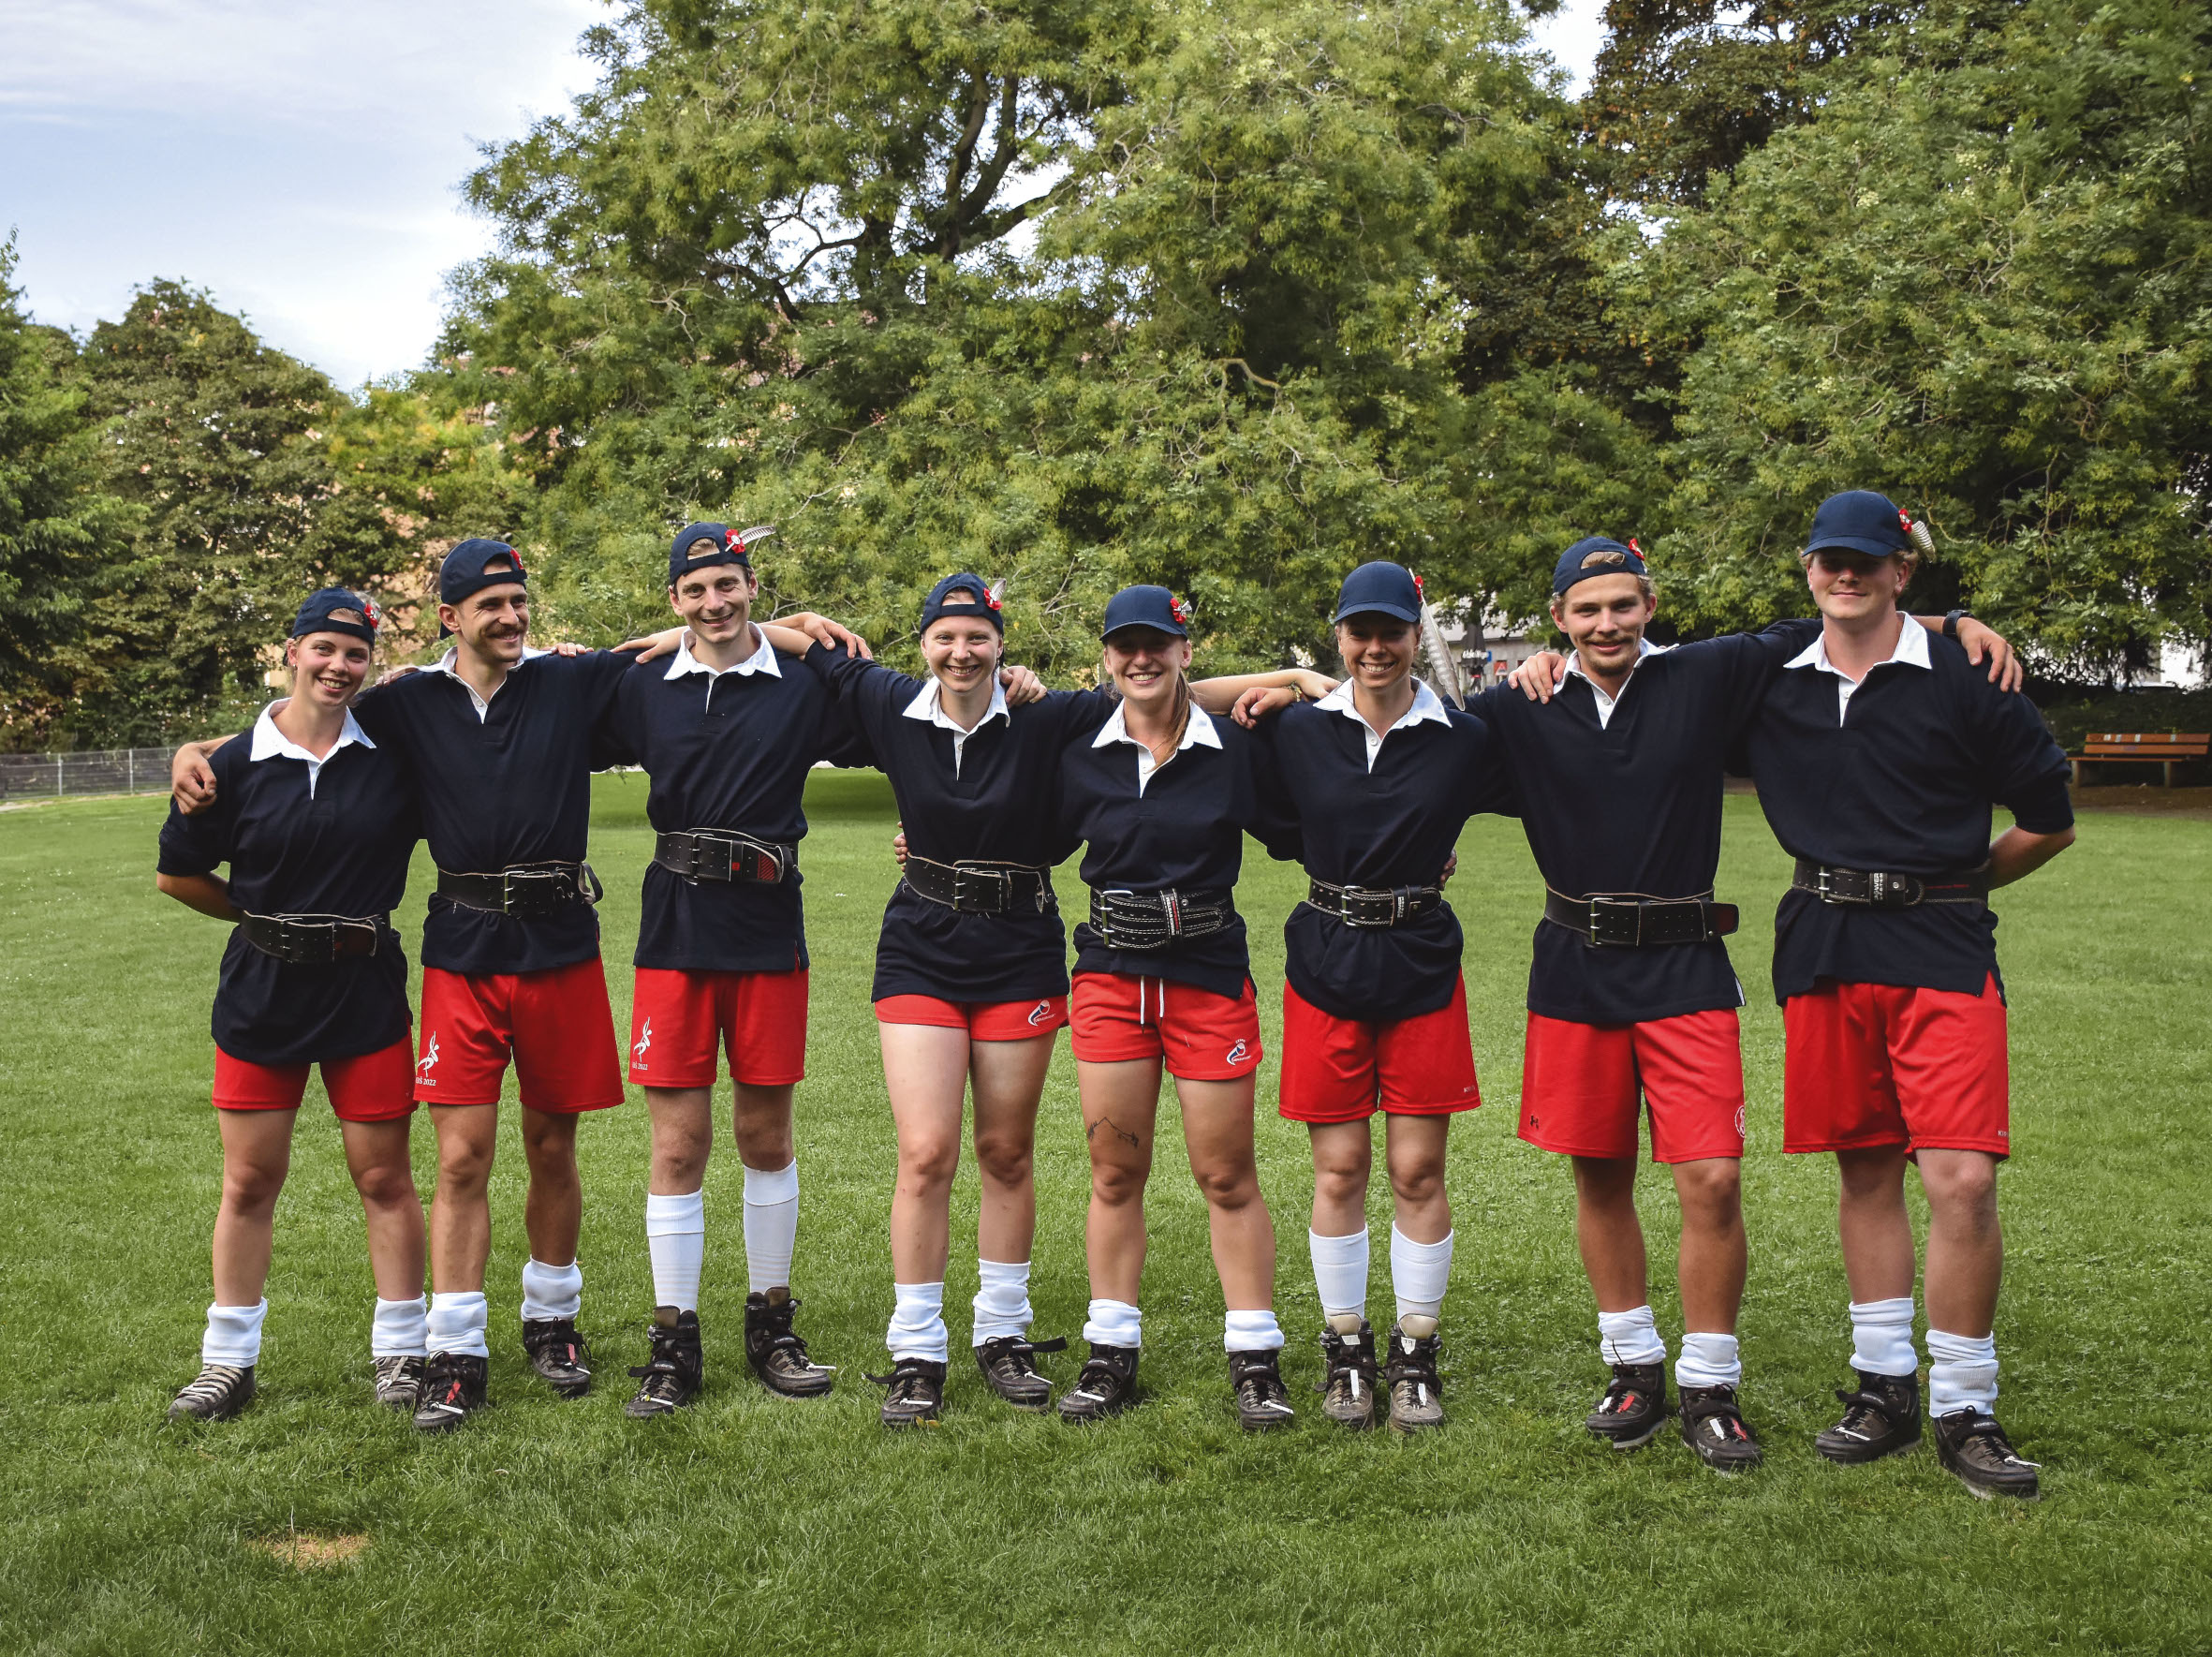
\includegraphics[width=\linewidth]{./lano-team-2.jpg}
\end{center}

Náš oddíl byl poprvé v~plné sokolské sestavě na soutěži venku, nemuseli jsme nikým doplňovat. Nabrali jsme zkušenost, která je ohromně cenná. Měli jsme veliké štěstí na možnost startovat ve více zápasech, než jsme na začátku vůbec doufali. Zatímco mistrům končí sezóna a k~lanu se vrátí zas až v~únoru, my trénovat nebudeme přestávat. Jako každý rok taháme ve čtvrtek od 20 h večer bez ohledu na počasí. 

Pořád nás může tahat víc, a tak jste mezi nás srdečně zváni. Můžete se společně s~námi stát průkopníky v~šíření u~nás dosti neznámého sportu a třeba vás tahání lana bude bavit tak jako nás.

\signature{Josef Kubišta}{}


% zadní obálka
\clearpage

\pagestyle{blank}
\newgeometry{margin=1cm}

\vspace*{96pt}

\pagecolor{sokolred}
\color{white}

\noindent {\fontsize{48pt}{56pt}\tyrs
se sokolským

\vspace*{24pt}

\noindent nazdar!}

\vspace*{\fill}

% \color{black}
\begin{center}
Vydává Tělocvičná jednota Sokol Libeň, Zenklova 37, Praha 8

\vspace*{12pt}

Na přípravě tohoto čísla se spolu s~autory jednotlivých textů podíleli:

grafická úprava – Martin Burian | jazyková úprava – Martina Waclawičová \\ editoři textů – Vít Jakoubek, Jan Přech
\end{center}

\end{document}